\documentclass[a4paper,12pt]{article}

% Packages
\usepackage[utf8]{inputenc}
\usepackage{amsmath}
\usepackage{amsfonts}
\usepackage{amssymb}
\usepackage{graphicx}
\usepackage{hyperref}
\usepackage{geometry}
\usepackage{booktabs}
\usepackage{subcaption}
\usepackage{float}
\usepackage{tabularx}

% Page Geometry
\geometry{a4paper, margin=1in}

% Title, Author, and Date
\title{Machine Learning Analysis on AVC and Salary Datasets}
\author{Dragomir Andrei}
\date{\today}

% Document
\begin{document}

\maketitle

\begin{abstract}
This document provides a comprehensive analysis of two machine learning models applied to the given datasets. The analysis includes data preprocessing, model training, evaluation, and comparison of results.
\end{abstract}

\newpage

\tableofcontents
\newpage

\section{Introduction}
In this analysis, we explore the Logistic Regression and the Multy Layer Perceptron models on the AVC and Salary datasets. The goal is to predict the target variable based on the features provided in the datasets.

\section*{Dataset Description}
\section{Medical and Lifestyle Information Dataset}

This dataset contains medical values and relevant lifestyle information for 5110 individuals. The dataset is intended to be used for predicting whether a person is likely to have a cerebrovascular accident (stroke) or not. The target attribute is \textit{cerebrovascular\_accident}, which has binary values indicating the presence (1) or absence (0) of a stroke. The classification task is binary.

The attributes in the dataset are as follows:

\begin{table}[H]
    \centering
    \caption{Attributes of the Medical and Lifestyle Information Dataset}
    \begin{tabular}{|l|l|p{10cm}|}
    \hline
    \textbf{Attribute} & \textbf{Type} & \textbf{Description} \\ \hline
    mean\_blood\_sugar\_level & numeric & The average blood sugar level over the observation period. \\ \hline
    cardiovascular\_issues & categorical & Indicates if the subject has a history of cardiovascular issues. Possible values: 0, 1. \\ \hline
    job\_category & categorical & The domain in which the person works. Possible values: child, entrepreneurial, N\_work\_history, private\_sector, public\_sector. \\ \hline
    body\_mass\_indicator & numeric & The body mass index indicating if the person is underweight, normal weight, overweight, or obese. \\ \hline
    sex & categorical & The gender of the person. Possible values: F, M. \\ \hline
    tobacco\_usage & categorical & Indicator for tobacco use, present or past. Possible values: ex-smoker, smoker, non-smoker. \\ \hline
    high\_blood\_pressure & categorical & Binary attribute indicating if a person suffers from high blood pressure. Possible values: 0, 1. \\ \hline
    married & categorical & Binary attribute indicating if the person has ever been married. Possible values: Y, N. \\ \hline
    living\_area & categorical & Type of area where the person has lived most of their life. Possible values: City, Countryside. \\ \hline
    years\_old & numeric & The age of the person in years. \\ \hline
    chaotic\_sleep & categorical & Binary attribute for an irregular sleep schedule. Possible values: 0, 1. \\ \hline
    analysis\_results & numeric & Results of the person's medical tests, which may include various measurements and health indicators. \\ \hline
    biological\_age\_index & numeric & An index estimating the biological age of a person based on various factors such as lifestyle and health status. \\ \hline
    cerebrovascular\_accident & categorical & Binary indicator of whether the person has had a stroke. Possible values: 0, 1. \\ \hline
    \end{tabular}
    \end{table}
    
\section{Employee Information Dataset}

This dataset contains personal, educational, and professional information of various employees. The objective of this dataset is the binary classification of employees into categories of earning above or below \$50K per year. The classification task is binary.

The attributes in the dataset are as follows:
\begin{table}[H]
\centering
\caption{Attributes of the Employee Information Dataset}
\begin{tabular}{|l|l|p{10cm}|}
\hline
\textbf{Attribute} & \textbf{Type} & \textbf{Description} \\ \hline
fnl & numeric & Socio-economic characteristic of the population from which the individual comes. \\ \hline
hpw & numeric & Number of hours worked per week. \\ \hline
relation & categorical & The type of relationship in which the individual is involved. \\ \hline
gain & numeric & Capital gain. \\ \hline
country & categorical & Country of origin. \\ \hline
job & categorical & The individual's occupation. \\ \hline
edu\_int & numeric & Number of years of education. \\ \hline
years & numeric & Age of the individual. \\ \hline
loss & numeric & Capital loss. \\ \hline
work\_type & categorical & Type of occupation. \\ \hline
partner & categorical & Type of partner the individual has. \\ \hline
edu & categorical & Type of education of the individual. \\ \hline
gender & categorical & Gender of the individual. \\ \hline
race & categorical & Race of the individual. \\ \hline
prod & numeric & Capital production. \\ \hline
gtype & categorical & Type of work contract. \\ \hline
\end{tabular}
\end{table}
    
\section{Attribute Type Identification}

Before utilizing a machine learning model for a dataset, it is crucial to identify the types of features in the dataset and their values. Understanding the nature of the attributes helps in selecting appropriate preprocessing techniques and models. The key distinctions among the types of attributes in the provided datasets are as follows:

\subsection{Continuous Numerical Attributes}

Continuous numerical attributes are features that can take any value within a given range. These attributes are measured on a continuous scale and can be divided into finer increments. Examples from the datasets include:

\begin{itemize}
    \item \textbf{mean\_blood\_sugar\_level}: Average blood sugar level measured over the observation period.
    \item \textbf{body\_mass\_indicator}: Body mass index indicating whether a person is underweight, normal weight, overweight, or obese.
    \item \textbf{years\_old}: Age of the person in years.
    \item \textbf{analysis\_results}: Results of medical tests.
    \item \textbf{biological\_age\_index}: An index estimating the biological age of a person based on various factors.
    \item \textbf{fnl}: Socio-economic characteristic of the population the individual comes from.
    \item \textbf{hpw}: Number of hours worked per week.
    \item \textbf{gain}: Capital gain.
    \item \textbf{edu\_int}: Number of years of education.
    \item \textbf{years}: Age of the individual.
    \item \textbf{loss}: Capital loss.
    \item \textbf{prod}: Capital production.
\end{itemize}

\subsection{Discrete Attributes}

Discrete attributes are features that take on a finite number of distinct values. These values are often categorical and can be counted in whole numbers. Examples from the datasets include:

\begin{itemize}
    \item \textbf{cardiovascular\_issues}: Whether the subject has a history of cardiovascular issues (0 or 1).
    \item \textbf{sex}: Gender of the person (F or M).
    \item \textbf{tobacco\_usage}: Indicator for smokers, either past or present (ex-smoker, smoker, non-smoker).
    \item \textbf{high\_blood\_pressure}: Indicator if a person has high blood pressure (0 or 1).
    \item \textbf{married}: Whether the person has ever been married (Y or N).
    \item \textbf{living\_area}: Type of area where the person has lived most of their life (City or Countryside).
    \item \textbf{chaotic\_sleep}: Indicator for an irregular sleep schedule (0 or 1).
    \item \textbf{cerebrovascular\_accident}: Indicator if the person has had a stroke (0 or 1).
    \item \textbf{relation}: Type of relationship the individual is involved in.
    \item \textbf{country}: Country of origin.
    \item \textbf{job}: Job of the individual.
    \item \textbf{work\_type}: Type of job.
    \item \textbf{partner}: Type of partner the individual has.
    \item \textbf{edu}: Type of education of the individual.
    \item \textbf{gender}: Gender of the individual.
    \item \textbf{race}: Race of the individual.
    \item \textbf{gtype}: Type of work contract.
    \item \textbf{job\_category}: Domain in which the person works.
\end{itemize}


Recognizing these distinctions helps in choosing the right methods for handling the data during preprocessing. For instance, continuous numerical attributes might require normalization or standardization, discrete attributes might need encoding, and ordinal attributes might need ordinal encoding to maintain the order information. Properly identifying and classifying the attributes ensures that the machine learning models can effectively learn from the data and make accurate predictions.

\section{Numeric Attributes Analysis}

In this section, we analyze the numeric attributes of the two datasets provided. The analysis includes the number of non-missing values, mean value, standard deviation, minimum value, 25th percentile, 50th percentile (median), 75th percentile, and maximum value for each numeric attribute.

\subsection{Healthcare Dataset}

\begin{table}[h!]
\centering
\caption{Statistics of Numeric Attributes in the Healthcare Dataset}
\vspace{0.5cm}
\small
\begin{tabularx}{\textwidth}{|l|X|X|X|X|X|X|X|X|}
\hline
\textbf{Attribute} & \textbf{No-miss} & \textbf{Mean} & \textbf{Std Dev} & \textbf{Min} & \textbf{25th Pctl} & \textbf{Mid} & \textbf{75th Pctl} & \textbf{Max} \\
\hline
mean\_blood\_sugar\_level & 5110 & 106.15 & 45.28 & 55.12 & 77.25 & 91.89 & 114.09 & 271.74 \\
body\_mass\_indicator & 4909 & 28.89 & 7.85 & 10.30 & 23.50 & 28.10 & 33.10 & 97.60 \\
years\_old & 5110 & 46.57 & 26.59 & 0.08 & 26.00 & 47.00 & 63.75 & 134.00 \\
analysis\_results & 4599 & 323.52 & 101.58 & 104.83 & 254.65 & 301.03 & 362.82 & 756.81 \\
biological\_age\_index & 5110 & 134.78 & 50.40 & -15.11 & 96.71 & 136.37 & 172.51 & 266.99 \\
\hline
\end{tabularx}
\normalsize
\end{table}

\textbf{Comments:}
\begin{itemize}
    \item The \textbf{mean\_blood\_sugar\_level} has a mean of 106.15 with a standard deviation of 45.28, indicating a wide range of values.
    \item The \textbf{body\_mass\_indicator} shows a mean of 28.89, suggesting that on average, individuals fall into the overweight category.
    \item The \textbf{years\_old} attribute ranges from 0.08 to 134 years, with a median of 47 years.
    \item The \textbf{analysis\_results} attribute has significant variability, as indicated by its standard deviation of 101.58.
    \item The \textbf{biological\_age\_index} has negative values, which may need to be investigated further for data correctness.
\end{itemize}

\subsection{Employee Dataset}

\begin{table}[h!]
\centering
\caption{Statistics of Numeric Attributes in the Employee Dataset}
\vspace{0.5cm}
\small
\begin{tabularx}{\textwidth}{|l|X|X|X|X|X|X|X|X|}
\hline
\textbf{Attribute} & \textbf{No-miss} & \textbf{Mean} & \textbf{Std Dev} & \textbf{Min} & \textbf{25th Pctl} & \textbf{Mid} & \textbf{75th Pctl} & \textbf{Max} \\
\hline
fnl & 9999 & 190352.9 & 106070.8 & 19214 & 118282.5 & 178472 & 237311 & 1455435 \\
hpw & 9199 & 40.42 & 12.52 & 1.0 & 40.0 & 40.0 & 45.0 & 99.0 \\
gain & 9999 & 979.85 & 7003.80 & 0.0 & 0.0 & 0.0 & 0.0 & 99999.0 \\
edu\_int & 9999 & 14.26 & 24.77 & 1.0 & 9.0 & 10.0 & 13.0 & 206.0 \\
years & 9999 & 38.65 & 13.75 & 17.0 & 28.0 & 37.0 & 48.0 & 90.0 \\
loss & 9999 & 84.11 & 394.04 & 0.0 & 0.0 & 0.0 & 0.0 & 3770.0 \\
prod & 9999 & 2014.93 & 14007.60 & -28.0 & 42.0 & 57.0 & 77.0 & 200125.0 \\
\hline
\end{tabularx}
\normalsize
\end{table}

\textbf{Comments:}
\begin{itemize}
    \item The \textbf{fnl} attribute has a high mean value and a wide range, indicating significant differences in the socio-economic status of individuals.
    \item The \textbf{hpw} (hours per week) attribute shows that most individuals work around 40 hours per week.
    \item The \textbf{gain} and \textbf{loss} attributes have a high standard deviation, indicating that only a few individuals have large capital gains or losses.
    \item The \textbf{edu\_int} (years of education) attribute shows that the majority of individuals have around 10 to 13 years of education.
    \item The \textbf{years} attribute shows an average age of around 38.65 years, with a minimum of 17 and a maximum of 90 years.
    \item The \textbf{prod} attribute has a high standard deviation, indicating variability in capital production.
\end{itemize}

\newpage

\section{Numeric Ranges for Attributes}

In this section, we present the boxplots for the numeric attributes in the datasets to visualize the distribution and identify any potential outliers.

\subsection{Healthcare Dataset}

\begin{figure}[h!]
    \centering
    \begin{subfigure}[b]{0.45\textwidth}
        \centering
        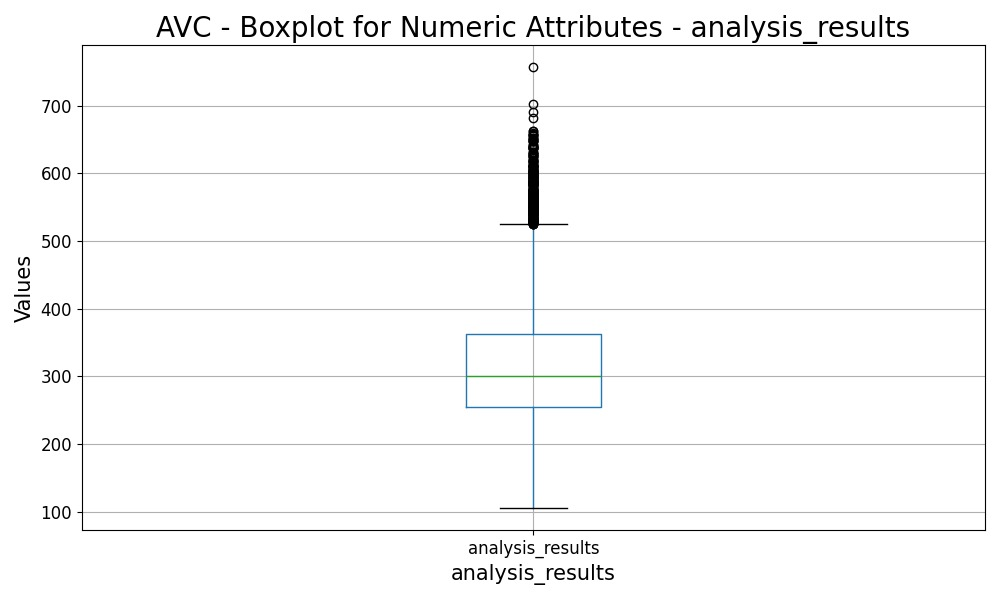
\includegraphics[width=\textwidth]{Resources/Boxplot_analysis_results.jpeg}
        \caption{Analysis Results}
        \label{fig:analysis_results}
    \end{subfigure}
    \hfill
    \begin{subfigure}[b]{0.45\textwidth}
        \centering
        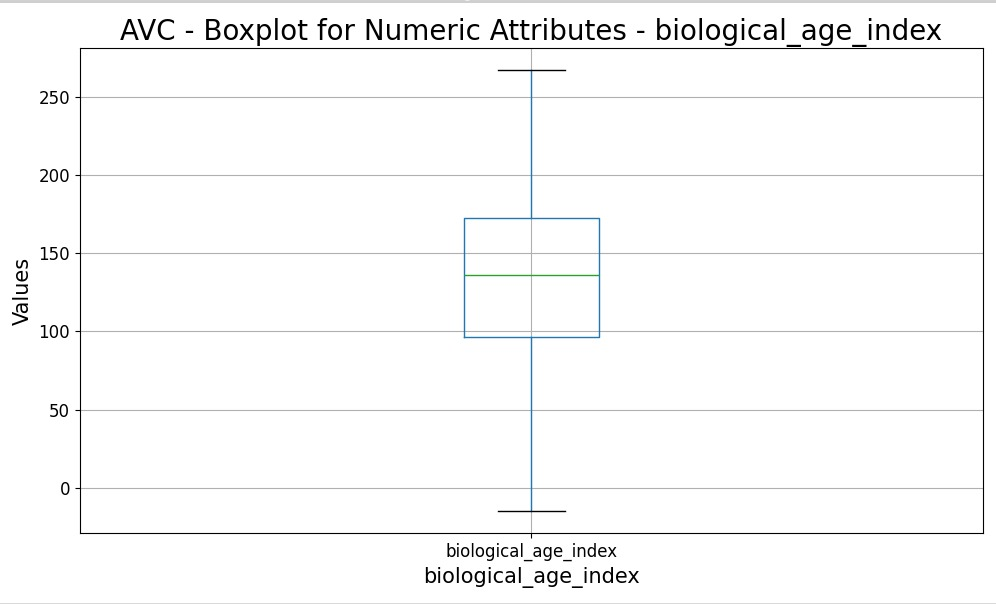
\includegraphics[width=\textwidth]{Resources/Boxplot_biological_index.jpeg}
        \caption{Biological Age Index}
        \label{fig:biological_index}
    \end{subfigure}
    
    \vspace{0.5cm}
    
    \begin{subfigure}[b]{0.45\textwidth}
        \centering
        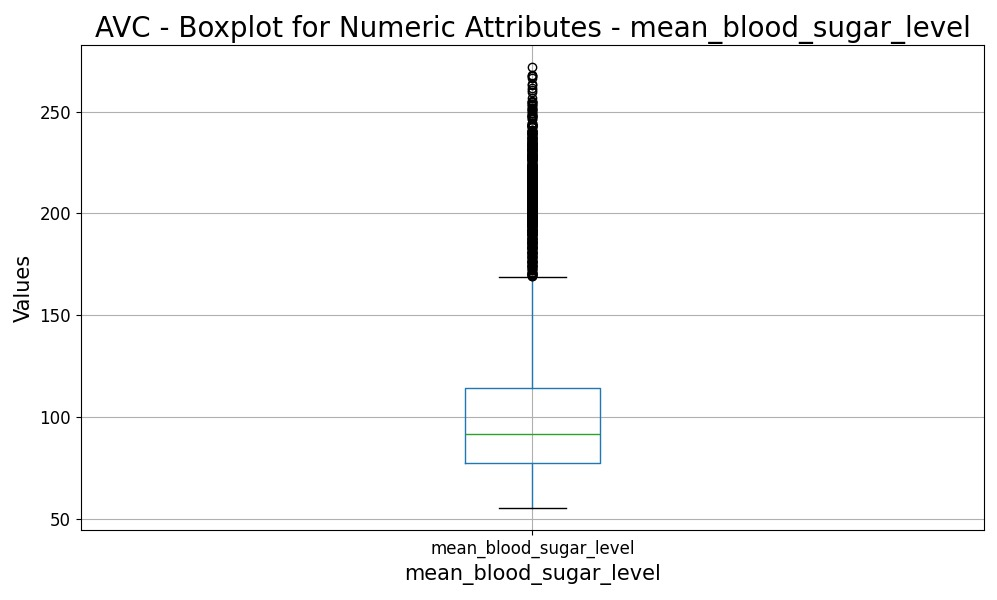
\includegraphics[width=\textwidth]{Resources/Boxplot_blood_sugar_level.jpeg}
        \caption{Mean Blood Sugar Level}
        \label{fig:blood_sugar_level}
    \end{subfigure}
    \hfill
    \begin{subfigure}[b]{0.45\textwidth}
        \centering
        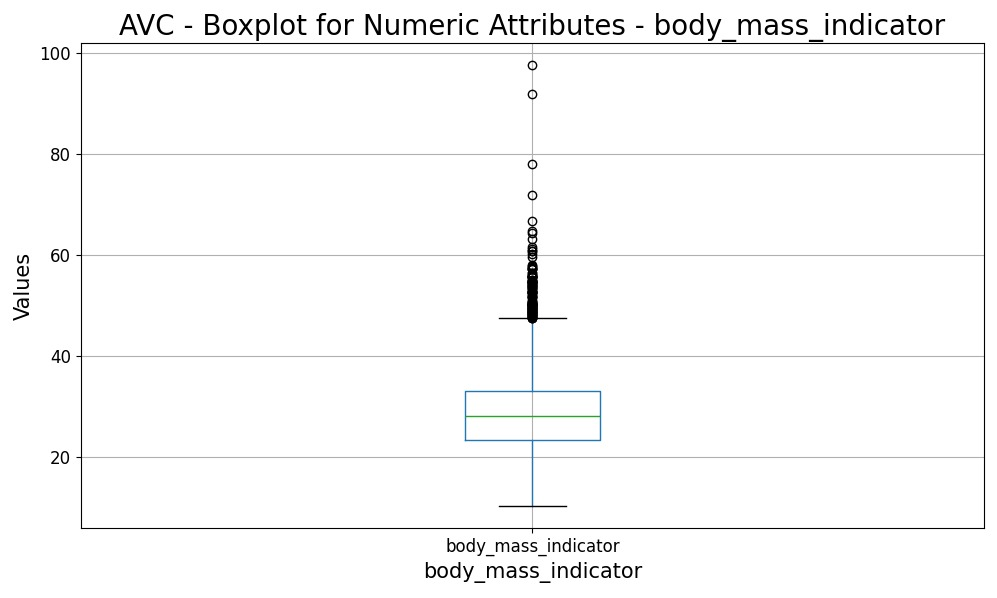
\includegraphics[width=\textwidth]{Resources/Boxplot_body_mass_indicator.jpeg}
        \caption{Body Mass Indicator}
        \label{fig:body_mass_indicator}
    \end{subfigure}
    
    \vspace{0.5cm}
    
    \begin{subfigure}[b]{0.45\textwidth}
        \centering
        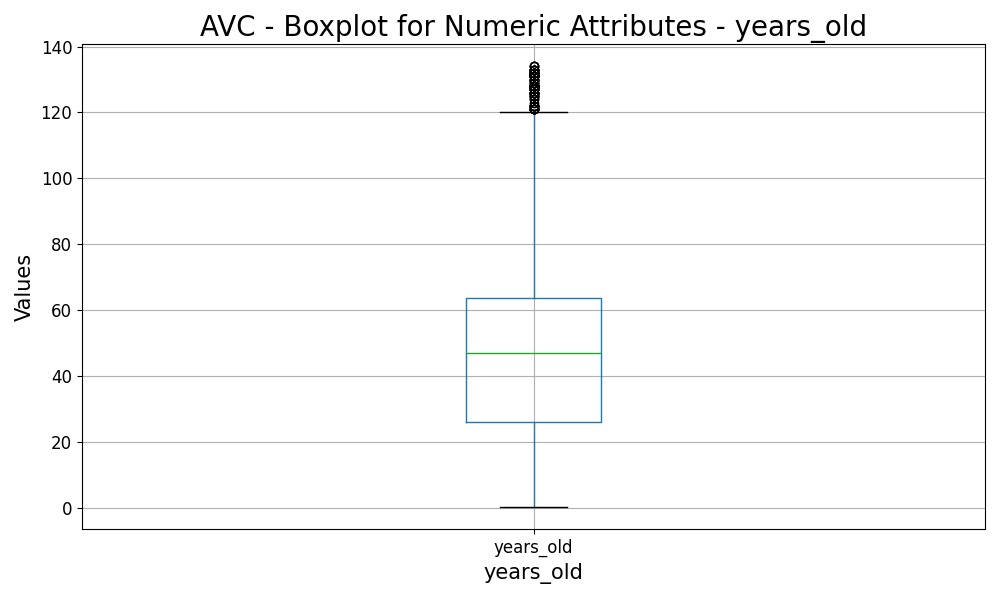
\includegraphics[width=\textwidth]{Resources/Boxplot_years_old.jpeg}
        \caption{Years Old}
        \label{fig:years_old}
    \end{subfigure}
    
    \caption{Boxplots for Healthcare Dataset Numeric Attributes}
\end{figure}

\newpage
\subsection{Employee Dataset}

\begin{figure}[h!]
    \centering
    \begin{subfigure}[b]{0.45\textwidth}
        \centering
        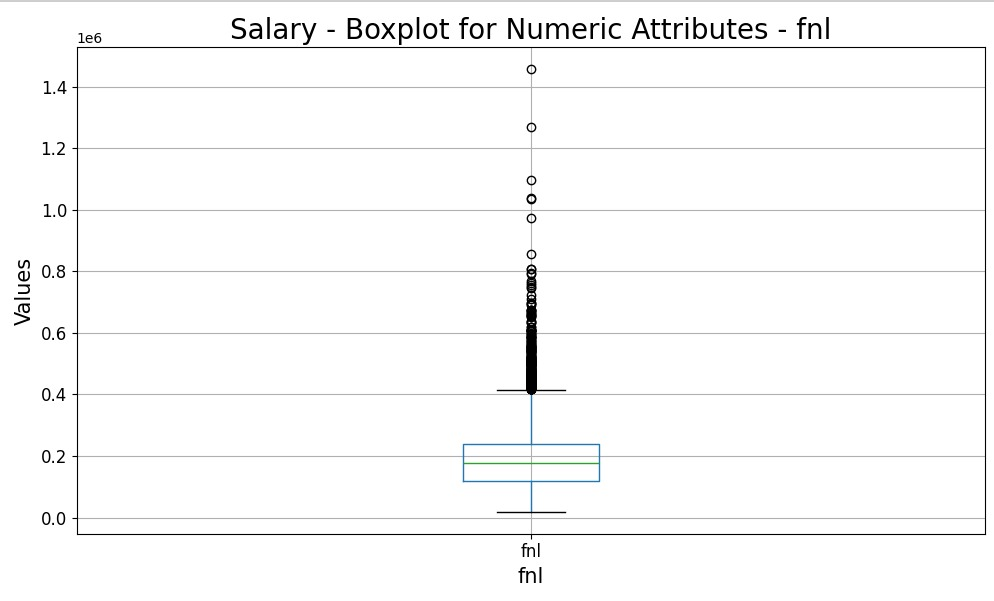
\includegraphics[width=\textwidth]{Resources/Boxplot_fnl.jpeg}
        \caption{FNL}
        \label{fig:fnl}
    \end{subfigure}
    \hfill
    \begin{subfigure}[b]{0.45\textwidth}
        \centering
        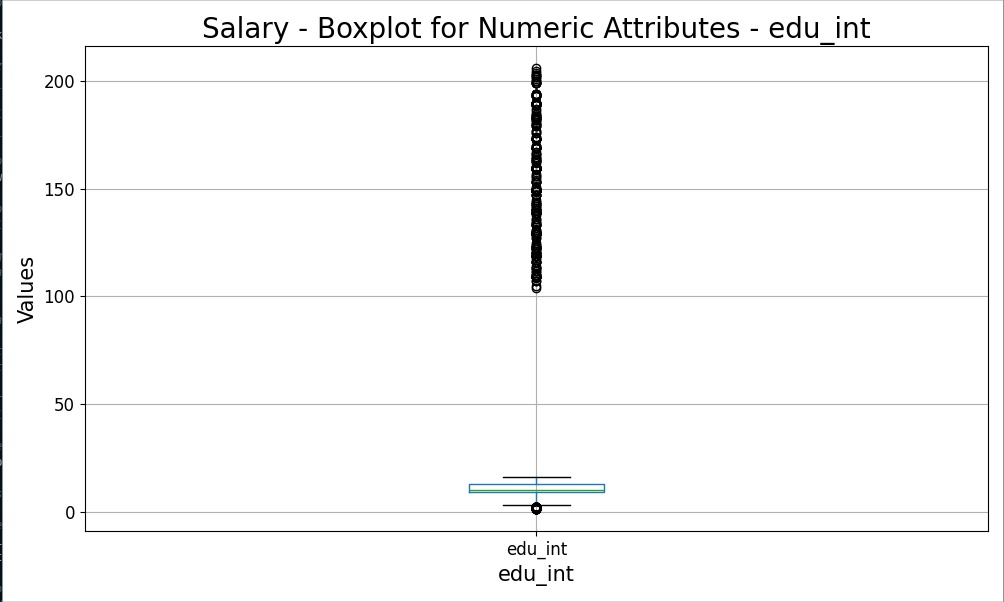
\includegraphics[width=\textwidth]{Resources/Boxplot_edu_int.jpeg}
        \caption{Education (Years)}
        \label{fig:edu_int}
    \end{subfigure}
    
    \vspace{0.5cm}
    
    \begin{subfigure}[b]{0.45\textwidth}
        \centering
        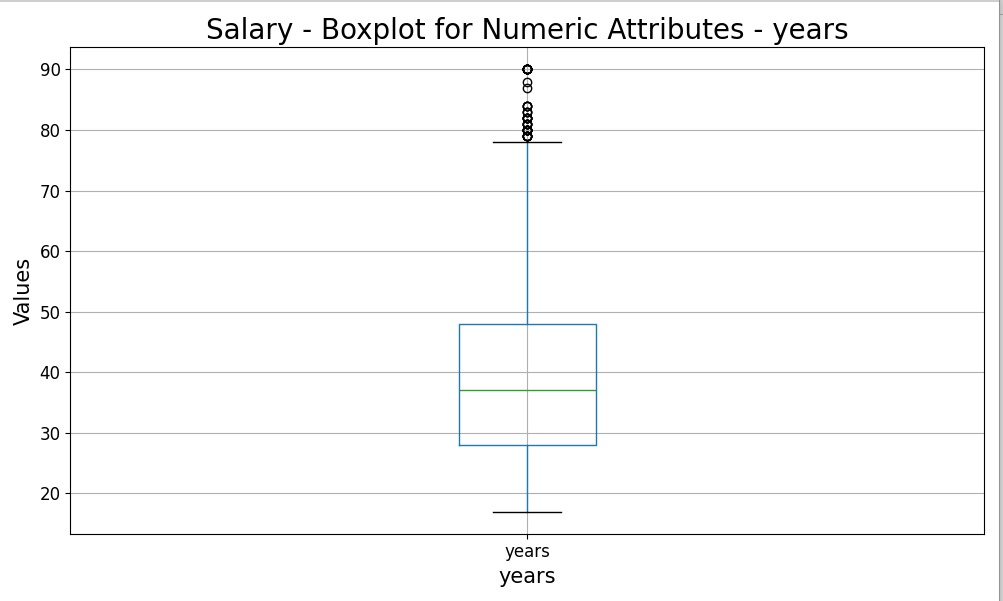
\includegraphics[width=\textwidth]{Resources/Boxplot_years.jpeg}
        \caption{Years}
        \label{fig:years}
    \end{subfigure}
    \hfill
    \begin{subfigure}[b]{0.45\textwidth}
        \centering
        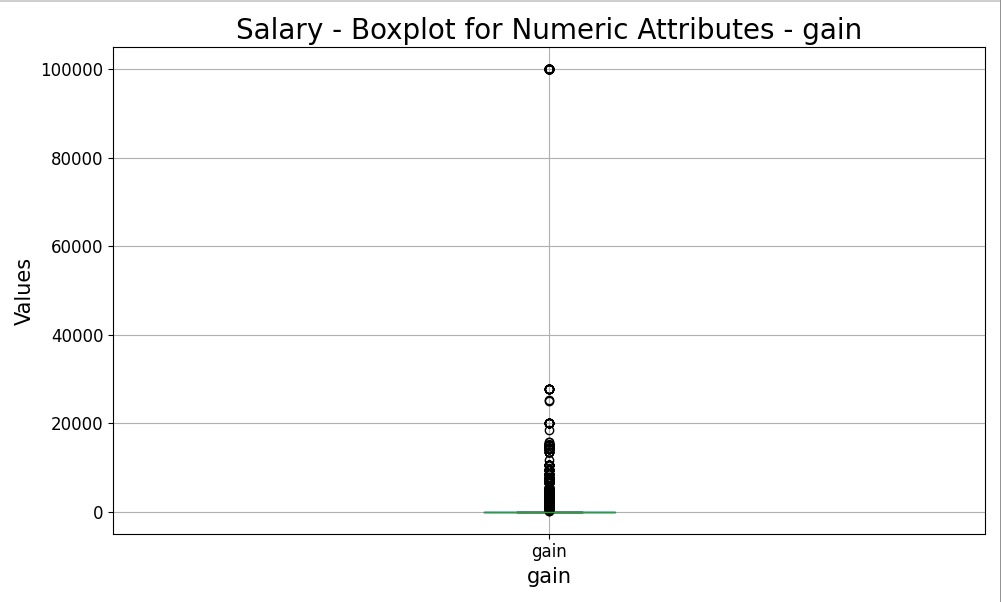
\includegraphics[width=\textwidth]{Resources/Boxplot_gain.jpeg}
        \caption{Gain}
        \label{fig:gain}
    \end{subfigure}
    
    \vspace{0.5cm}
    
    \begin{subfigure}[b]{0.45\textwidth}
        \centering
        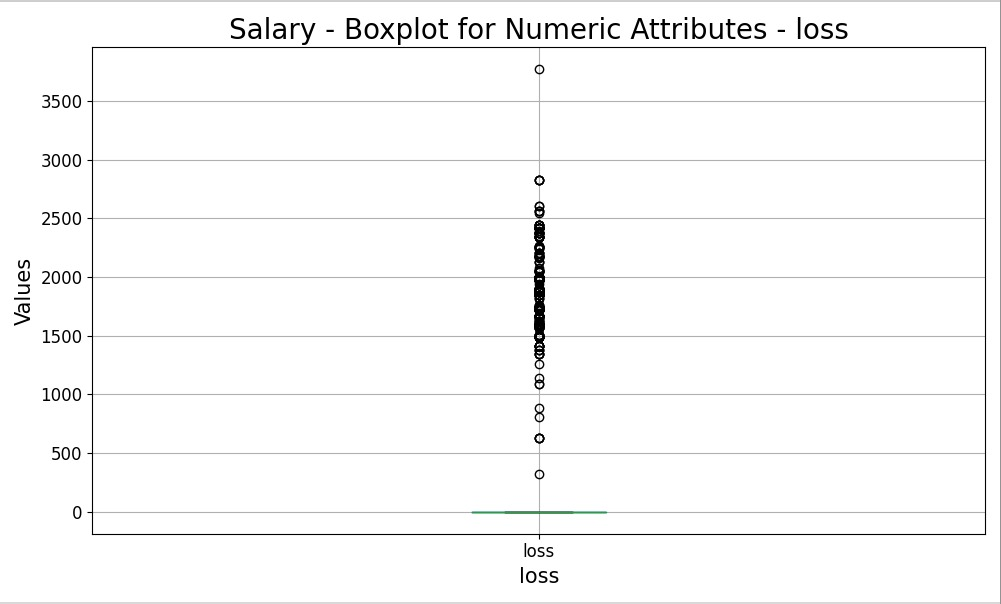
\includegraphics[width=\textwidth]{Resources/Boxplot_loss.jpeg}
        \caption{Loss}
        \label{fig:loss}
    \end{subfigure}
    \hfill
    \begin{subfigure}[b]{0.45\textwidth}
        \centering
        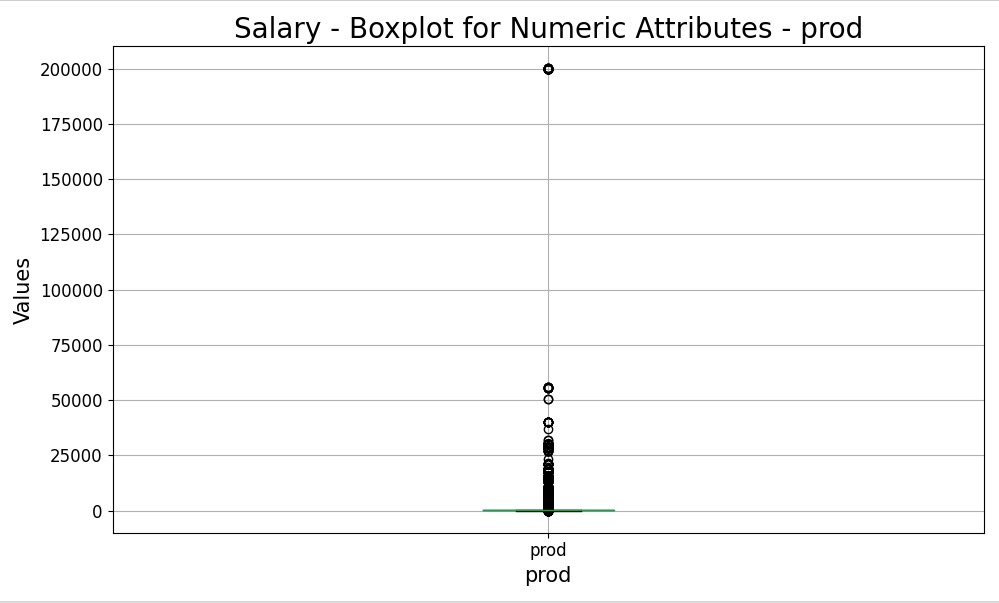
\includegraphics[width=\textwidth]{Resources/Boxplot_prod.jpeg}
        \caption{Prod}
        \label{fig:prod}
    \end{subfigure}
    
    \caption{Boxplots for Employee Dataset Numeric Attributes}
\end{figure}

\newpage

\section{Categorical Attributes Analysis}

In this section, we analyze the categorical attributes of the datasets. The tables below present the attributes along with the number of non-missing values and the number of unique values for each attribute.

\subsection{Healthcare Dataset}

\begin{table}[h!]
\centering
\caption{Categorical Attributes - Healthcare Dataset}
\vspace{0.5cm}
\small
\begin{tabularx}{\textwidth}{|l|X|X|}
\hline
\textbf{Attribute} & \textbf{Number of Non-Missing Values} & \textbf{Number of Unique Values} \\ \hline
cardiovascular\_issues & 5110 & 2 \\ \hline
job\_category & 5110 & 5 \\ \hline
sex & 5110 & 2 \\ \hline
tobacco\_usage & 5110 & 4 \\ \hline
high\_blood\_pressure & 5110 & 2 \\ \hline
married & 4599 & 2 \\ \hline
living\_area & 5110 & 2 \\ \hline
chaotic\_sleep & 5110 & 2 \\ \hline
cerebrovascular\_accident & 5110 & 2 \\ \hline
\end{tabularx}
\normalsize
\end{table}

\subsection{Employee Dataset}

\begin{table}[h!]
\centering
\caption{Categorical Attributes - Employee Dataset}
\vspace{0.5cm}
\small
\begin{tabularx}{\textwidth}{|l|X|X|}
\hline
\textbf{Attribute} & \textbf{Number of Non-Missing Values} & \textbf{Number of Unique Values} \\ \hline
relation & 9999 & 6 \\ \hline
country & 9999 & 41 \\ \hline
job & 9999 & 14 \\ \hline
work\_type & 9999 & 9 \\ \hline
partner & 9999 & 7 \\ \hline
edu & 9999 & 16 \\ \hline
gender & 9199 & 2 \\ \hline
race & 9999 & 5 \\ \hline
gtype & 9999 & 2 \\ \hline
money & 9999 & 2 \\ \hline
\end{tabularx}
\normalsize
\end{table}

\newpage
\subsection{Comments}

The healthcare dataset includes several categorical attributes such as `cardiovascular\_issues`, `job\_category`, `sex`, and `tobacco\_usage`. Each of these attributes has a varying number of unique values, indicating different levels of categorization. For instance, `tobacco\_usage` has four unique values, while `sex` has only two. It is also noted that the `married` attribute has fewer non-missing values compared to others, which might require special handling during data preprocessing.

The employee dataset, on the other hand, contains a wider range of categorical attributes with a larger variety of unique values, especially for `country` and `edu`, which have 41 and 16 unique values, respectively. Attributes like `gender` and `gtype` are binary, which simplifies their processing. The variety in the number of unique values across different attributes in both datasets indicates the complexity and diversity of the data, which must be carefully considered during the feature engineering and model building stages.

\section{Categorical Distribution for Attributes}

\subsection{Healthcare Dataset}
\begin{figure}[H]
    \centering
    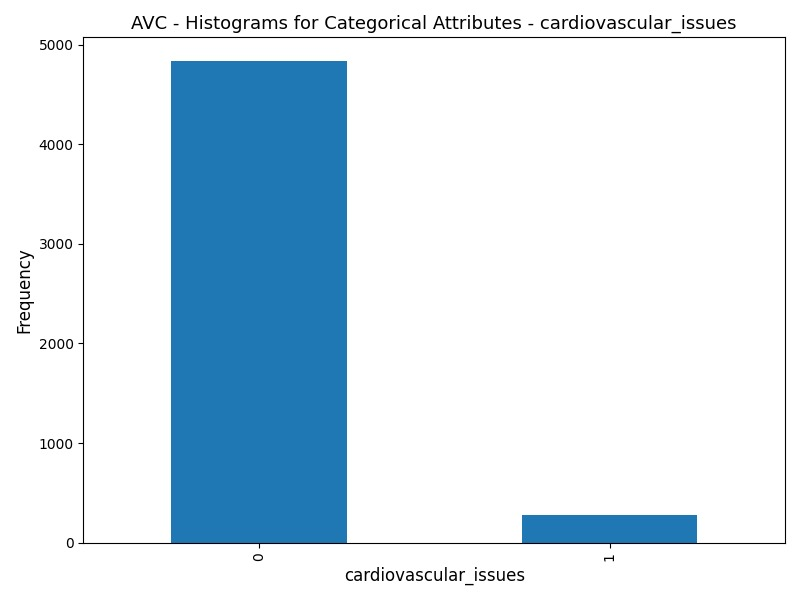
\includegraphics[width=0.8\textwidth]{Resources/histogram_cardio_issues.jpeg}
    \caption{Cardiovascular Issues}
\end{figure}

\begin{figure}[H]
    \centering
    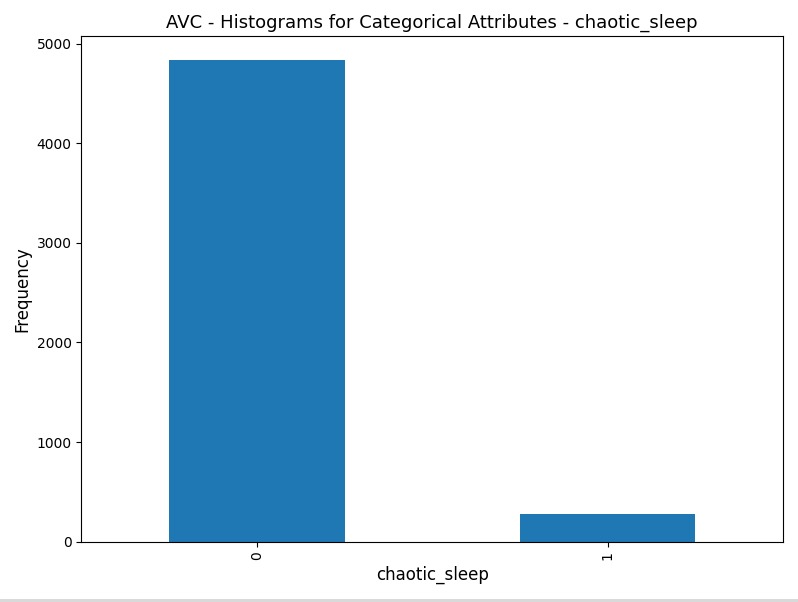
\includegraphics[width=0.8\textwidth]{Resources/histogram_chaotic_sleep.jpeg}
    \caption{Chaotic Sleep}
\end{figure}

\begin{figure}[H]
    \centering
    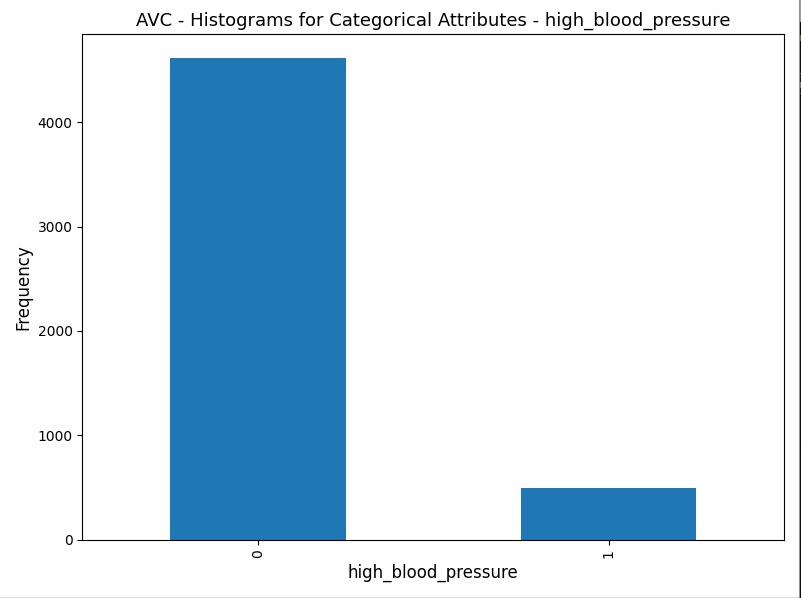
\includegraphics[width=0.8\textwidth]{Resources/histogram_high_blood_pressure.jpeg}
    \caption{High Blood Pressure}
\end{figure}

\begin{figure}[H]
    \centering
    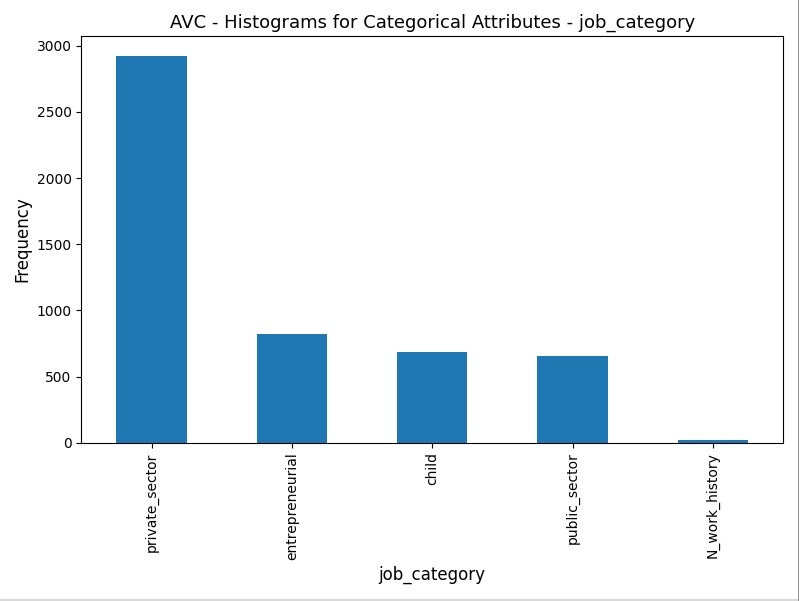
\includegraphics[width=0.8\textwidth]{Resources/histogram_job_cat.jpeg}
    \caption{Job Category}
\end{figure}

\begin{figure}[H]
    \centering
    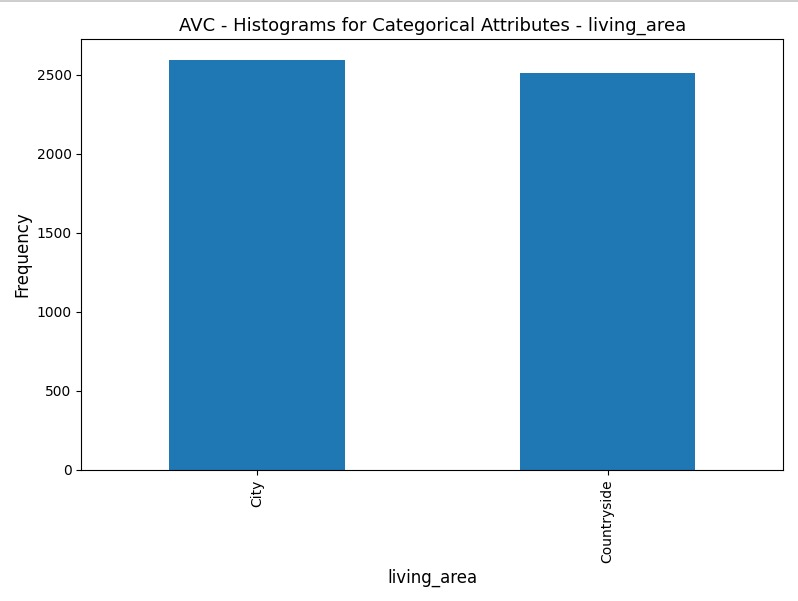
\includegraphics[width=0.8\textwidth]{Resources/histogram_living_area.jpeg}
    \caption{Living Area}
\end{figure}

\begin{figure}[H]
    \centering
    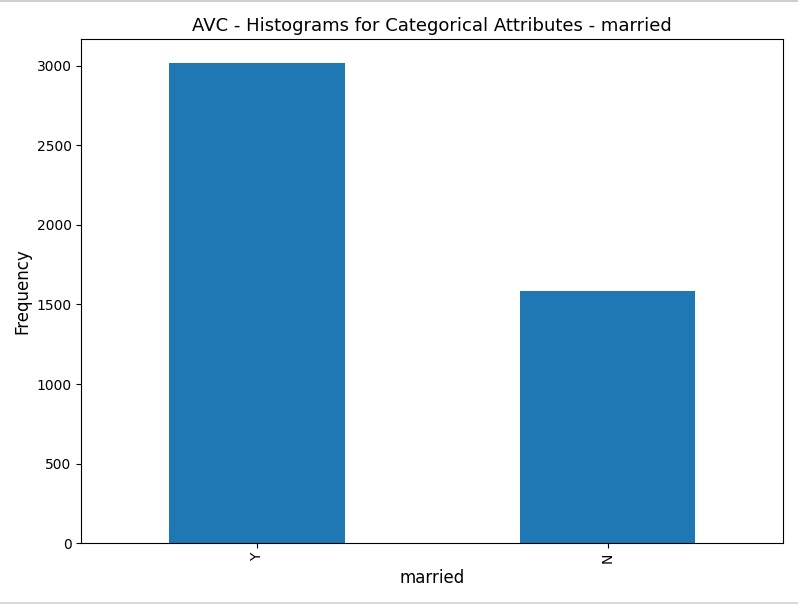
\includegraphics[width=0.8\textwidth]{Resources/histogram_married.jpeg}
    \caption{Married}
\end{figure}

\begin{figure}[H]
    \centering
    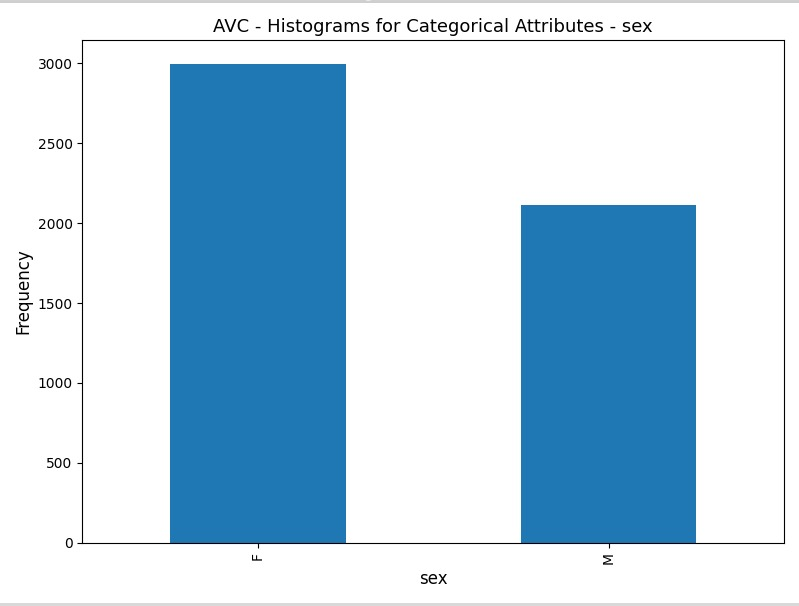
\includegraphics[width=0.8\textwidth]{Resources/histogram_sex.jpeg}
    \caption{Sex}
\end{figure}

\begin{figure}[H]
    \centering
    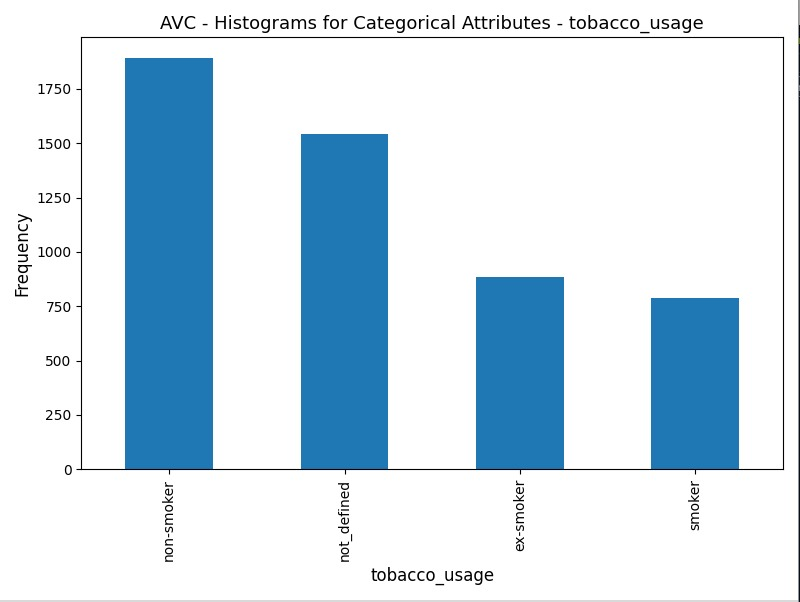
\includegraphics[width=0.8\textwidth]{Resources/histogram_tobacco_usage.jpeg}
    \caption{Tobacco Usage}
\end{figure}

\subsection{Salary Dataset}
\begin{figure}[H]
    \centering
    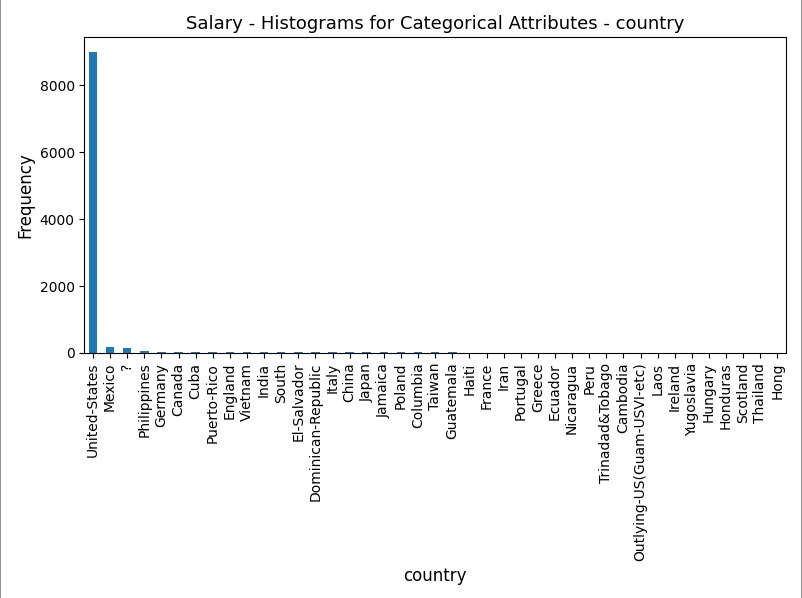
\includegraphics[width=0.8\textwidth]{Resources/histogram_country.jpeg}
    \caption{Country}
\end{figure}

\begin{figure}[H]
    \centering
    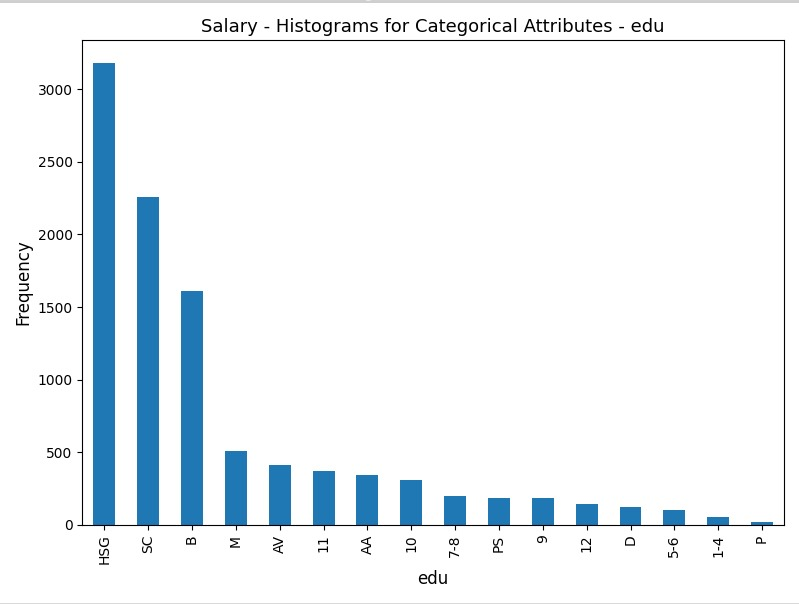
\includegraphics[width=0.8\textwidth]{Resources/histogram_edu.jpeg}
    \caption{Education}
\end{figure}

\begin{figure}[H]
    \centering
    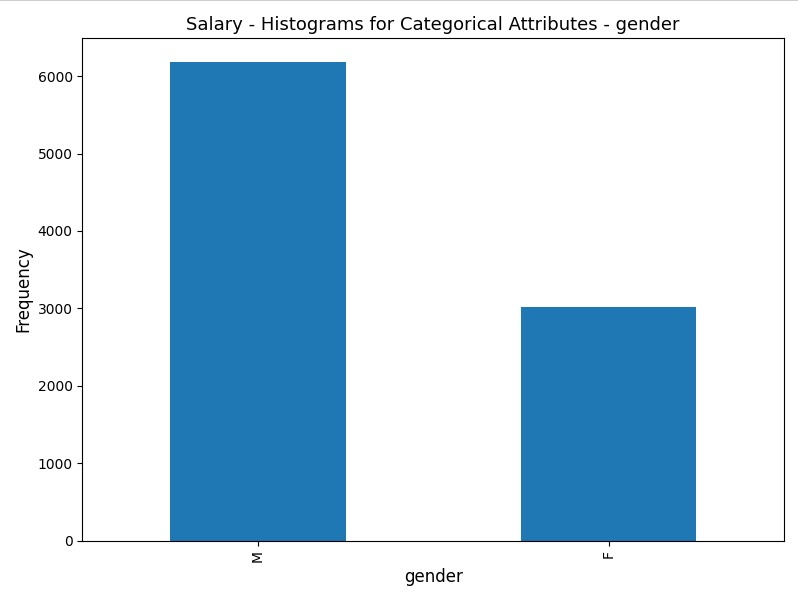
\includegraphics[width=0.8\textwidth]{Resources/histogram_gender.jpeg}
    \caption{Gender}
\end{figure}

\begin{figure}[H]
    \centering
    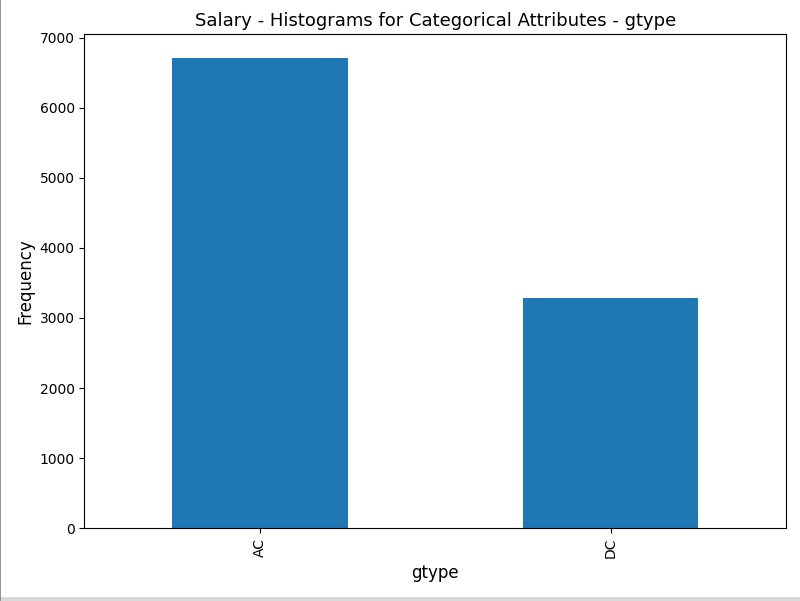
\includegraphics[width=0.8\textwidth]{Resources/histogram_gtype.jpeg}
    \caption{Job Type}
\end{figure}

\begin{figure}[H]
    \centering
    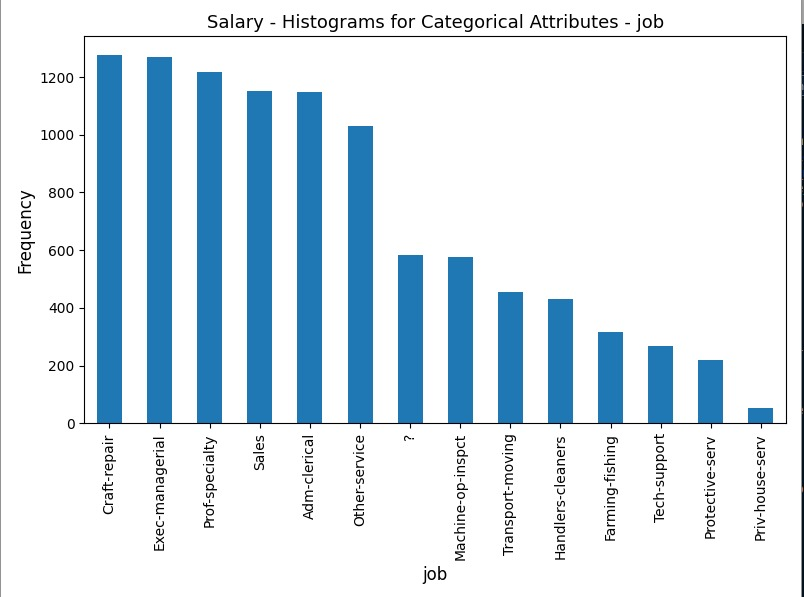
\includegraphics[width=0.8\textwidth]{Resources/histogram_job.jpeg}
    \caption{Job}
\end{figure}

\begin{figure}[H]
    \centering
    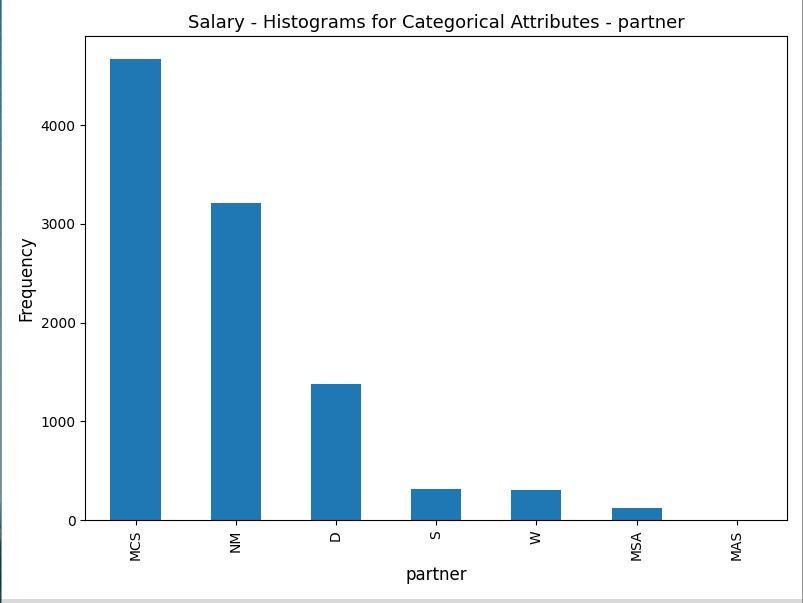
\includegraphics[width=0.8\textwidth]{Resources/histogram_partner.jpeg}
    \caption{Partner}
\end{figure}

\begin{figure}[H]
    \centering
    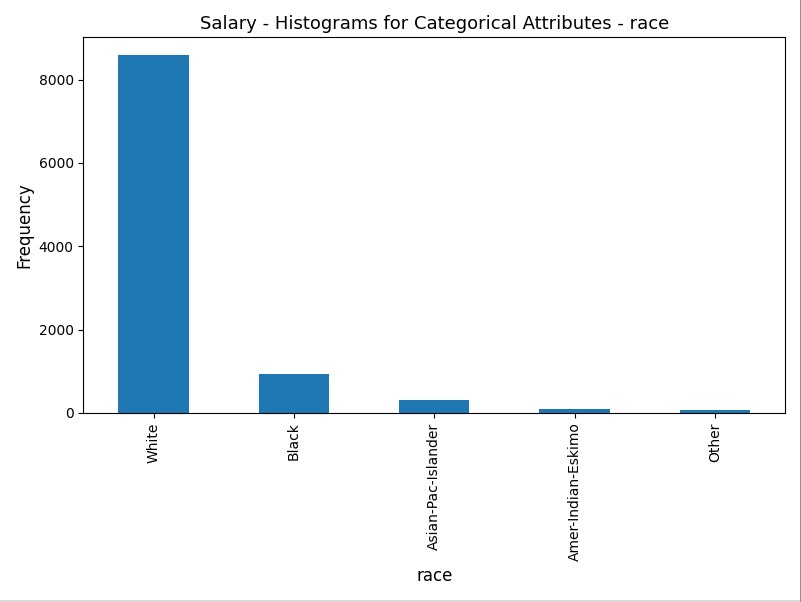
\includegraphics[width=0.8\textwidth]{Resources/histogram_race.jpeg}
    \caption{Race}
\end{figure}

\begin{figure}[H]
    \centering
    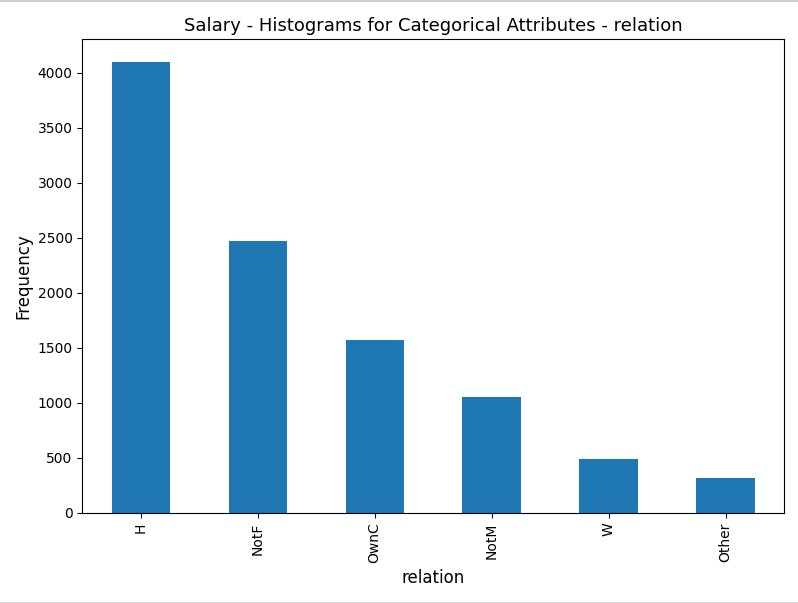
\includegraphics[width=0.8\textwidth]{Resources/histogram_relation.jpeg}
    \caption{Relation}
\end{figure}

\begin{figure}[H]
    \centering
    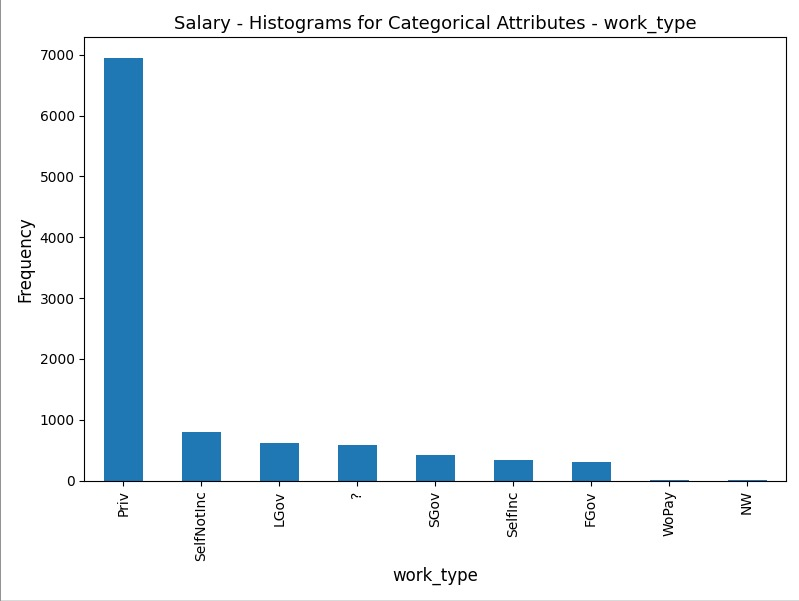
\includegraphics[width=0.8\textwidth]{Resources/histogram_work_type.jpeg}
    \caption{Work Type}
\end{figure}

\newpage

\section{Class Balance}
This section presents the class balance for both the AVC and Salary datasets. The class balance is an important aspect to consider as it influences the evaluation metrics we should focus on.

\subsection{AVC Dataset}
\begin{figure}[h!]
    \centering
    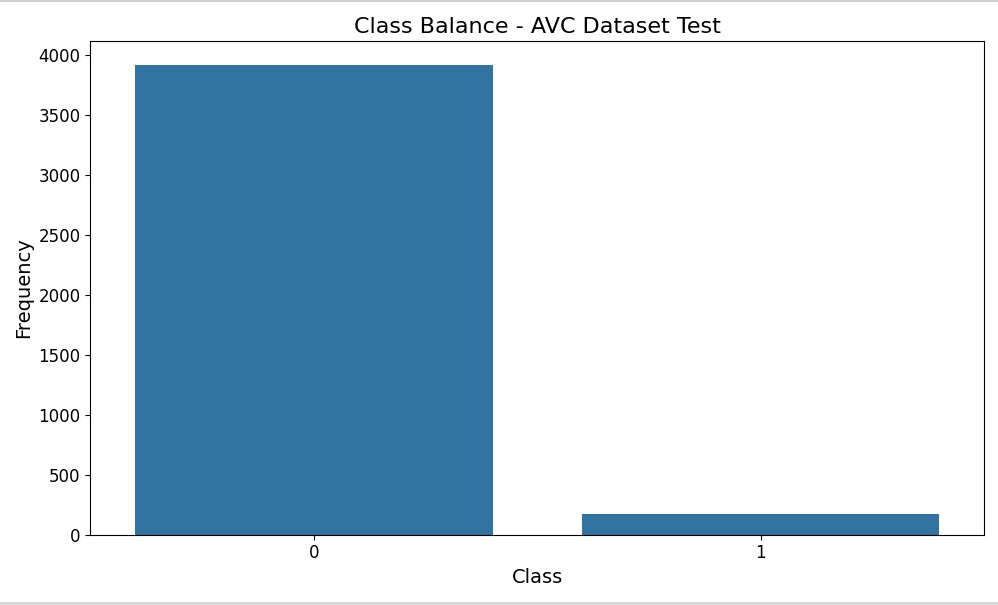
\includegraphics[width=0.8\textwidth]{Resources/class_balance_avc_test.jpeg}
    \caption{Class Balance - AVC Dataset Test}
\end{figure}

\begin{figure}[h!]
    \centering
    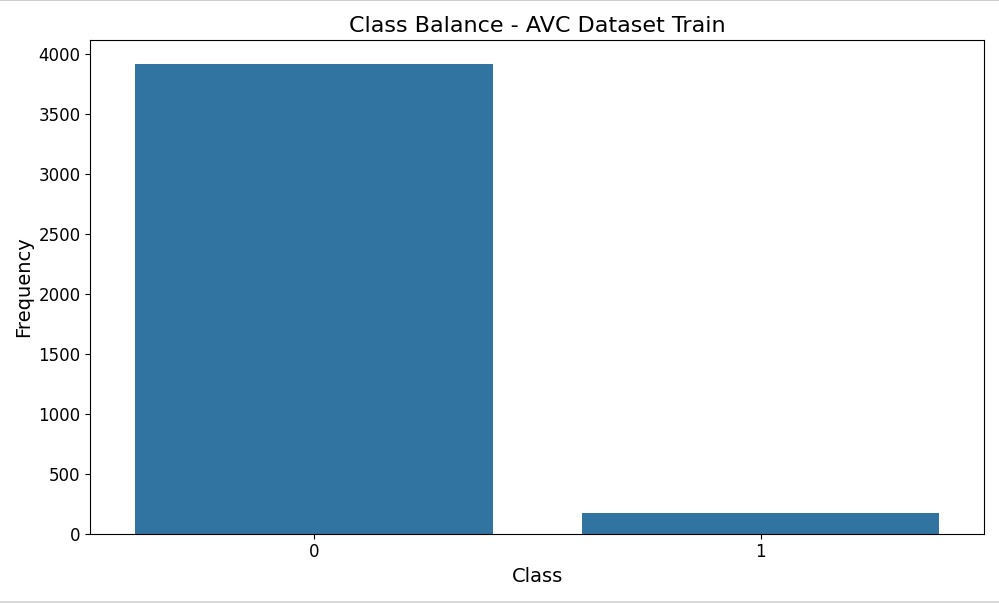
\includegraphics[width=0.8\textwidth]{Resources/class_balance_avc_train.jpeg}
    \caption{Class Balance - AVC Dataset Train}
\end{figure}


\newpage

\subsection{Salary Dataset}
\begin{figure}[h!]
    \centering
    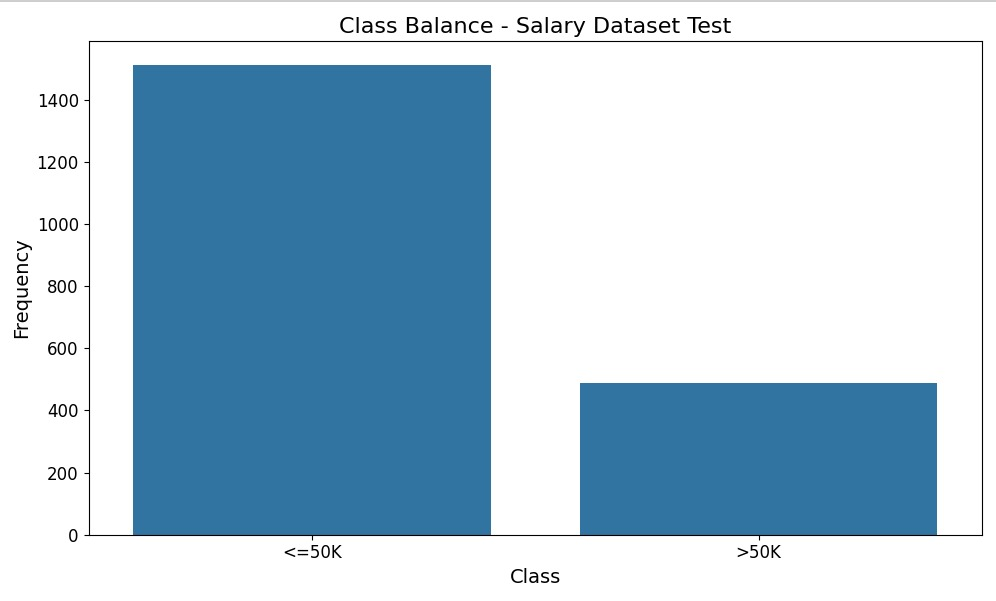
\includegraphics[width=0.8\textwidth]{Resources/class_balance_salary_test.jpeg}
    \caption{Class Balance - Salary Dataset Test}
\end{figure}

\begin{figure}[h!]
    \centering
    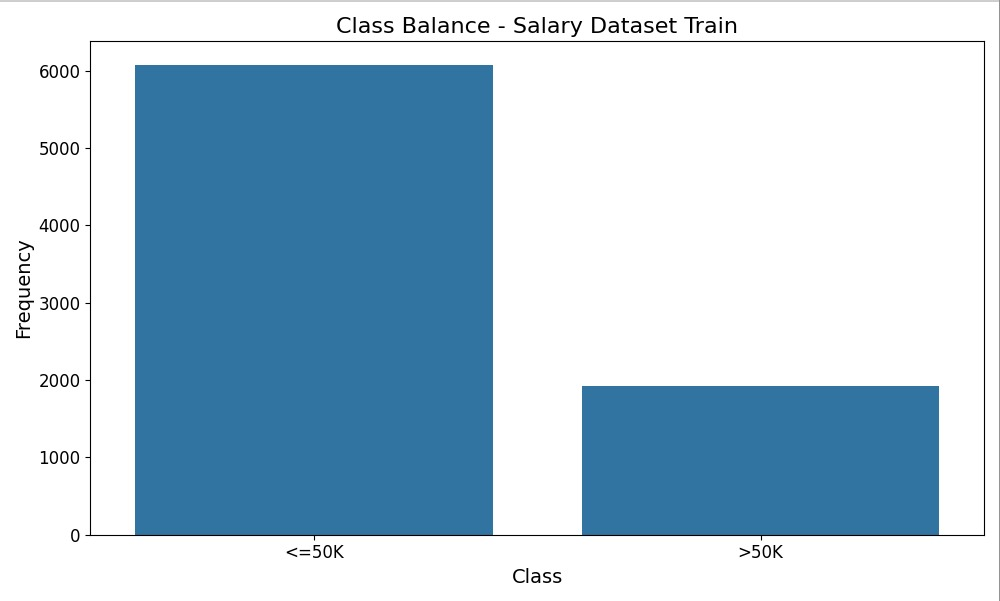
\includegraphics[width=0.8\textwidth]{Resources/class_balance_salary_train.jpeg}
    \caption{Class Balance - Salary Dataset Train}
\end{figure}

\subsection{Comments}
From the class balance plots above, it is evident that both datasets exhibit significant class imbalance. In the AVC dataset, the majority class (no stroke) is much more prevalent than the minority class (stroke). Similarly, in the Salary dataset, the class of individuals earning less than or equal to 50K is more common than the class of individuals earning more than 50K.

Class imbalance can have a substantial impact on model performance and evaluation. Models may become biased towards the majority class, leading to poor performance on the minority class. To address this, it is crucial to focus on evaluation metrics that provide a better understanding of performance on imbalanced datasets. Specifically, we should emphasize:

\begin{itemize}
    \item \textbf{F1 Score}: The harmonic mean of precision and recall, which provides a balance between the two.
    \item \textbf{Precision}: The ability of the classifier to not label a negative sample as positive.
    \item \textbf{Recall}: The ability of the classifier to find all positive samples.
\end{itemize}

By prioritizing these metrics, we can better assess and compare the performance of different algorithms on these imbalanced datasets.

\newpage

\section{Attribute Correlation}
This section presents the correlation matrices for both the AVC and Salary datasets. The correlation matrices are split into numerical and categorical attributes for both train and test sets.

\subsection{AVC Dataset}
\subsubsection{Numerical Attributes}
\begin{figure}[h!]
    \centering
    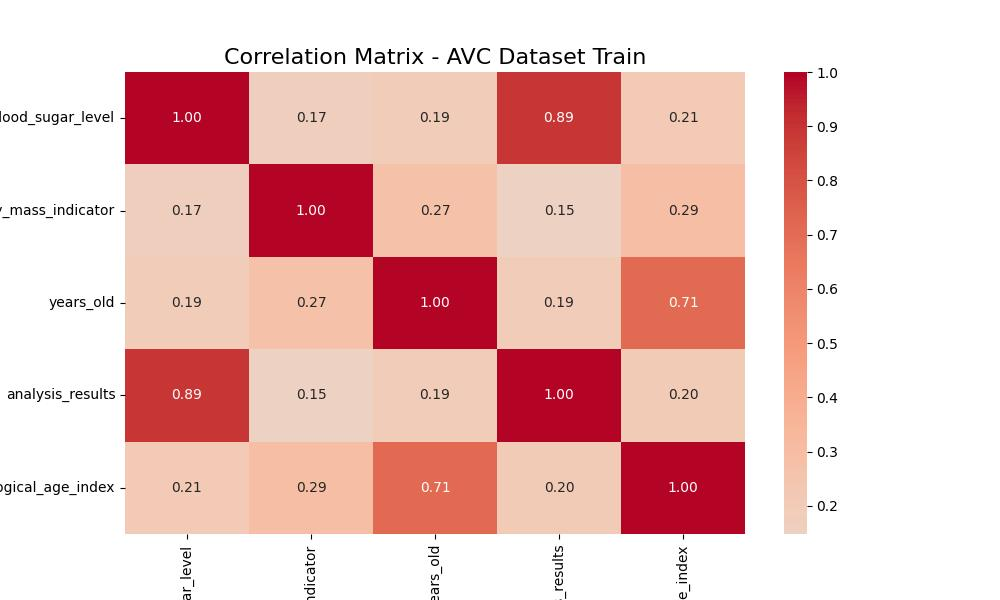
\includegraphics[width=0.8\textwidth]{Resources/matrix_avc_train.jpeg}
    \caption{Correlation Matrix - Numerical Attributes - AVC Dataset Train}
\end{figure}

\begin{figure}[h!]
    \centering
    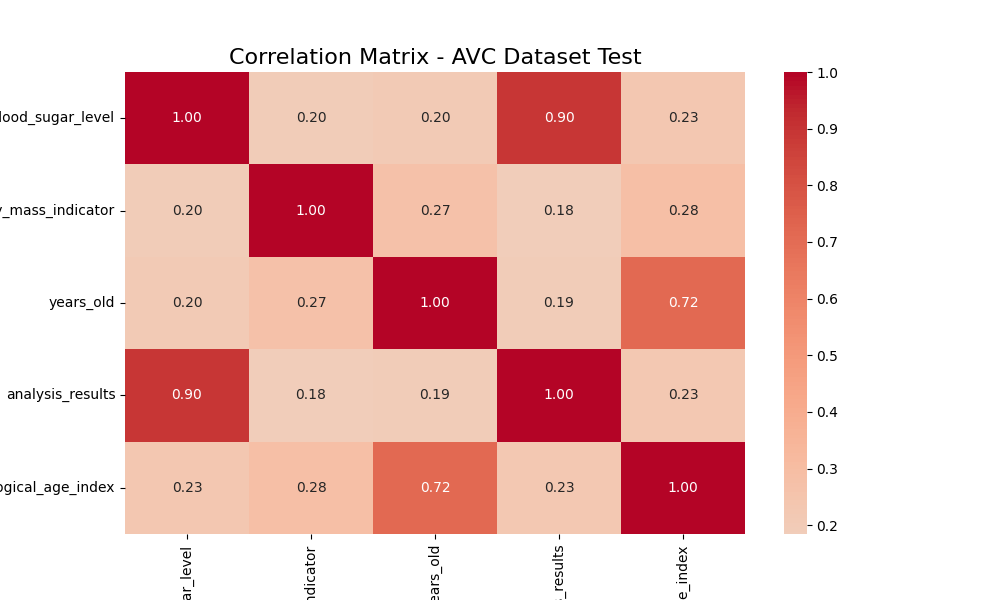
\includegraphics[width=0.8\textwidth]{Resources/matrix_avc_test.png}
    \caption{Correlation Matrix - Numerical Attributes - AVC Dataset Test}
\end{figure}

\newpage
\subsubsection{Categorical Attributes}
\begin{figure}[h!]
    \centering
    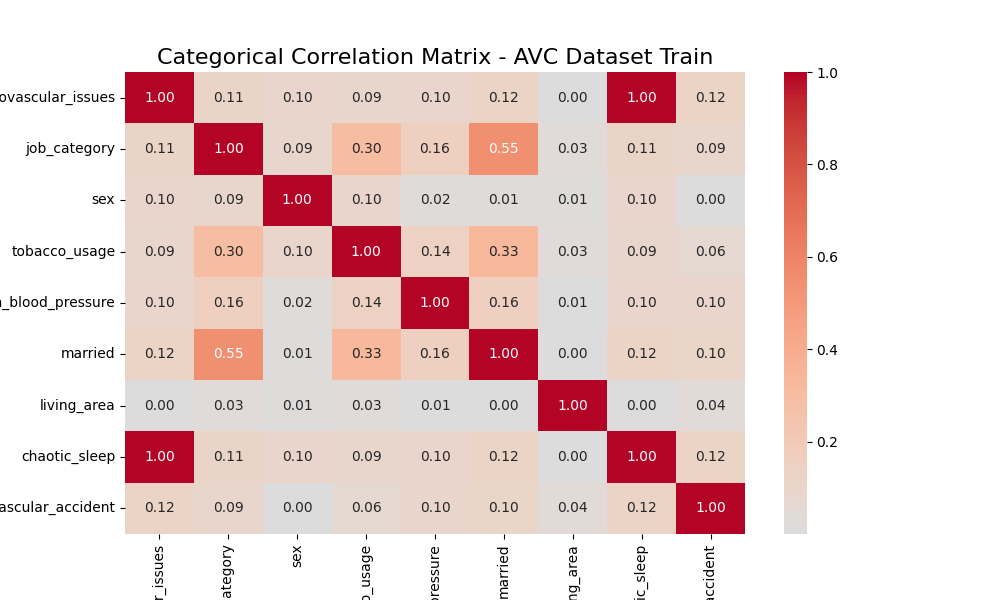
\includegraphics[width=0.8\textwidth]{Resources/matrix_categorial_avc_train.png}
    \caption{Categorical Correlation Matrix - AVC Dataset Train}
\end{figure}

\begin{figure}[h!]
    \centering
    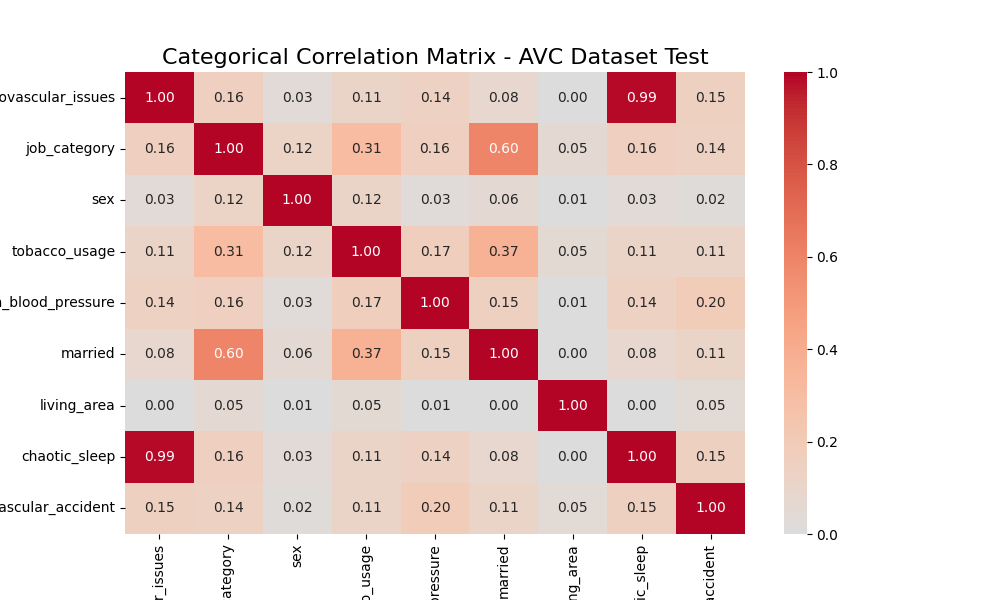
\includegraphics[width=0.8\textwidth]{Resources/matrix_categorial_avc_test.png}
    \caption{Categorical Correlation Matrix - AVC Dataset Test}
\end{figure}

\newpage
\subsection{Salary Dataset}
\subsubsection{Numerical Attributes}
\begin{figure}[h!]
    \centering
    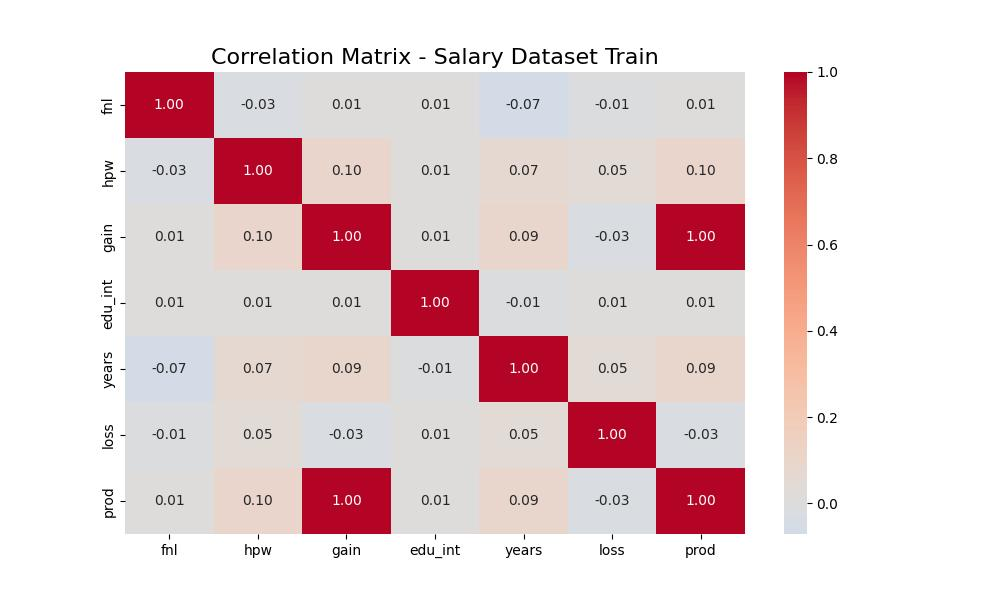
\includegraphics[width=0.8\textwidth]{Resources/matrix_salary_train.jpeg}
    \caption{Correlation Matrix - Numerical Attributes - Salary Dataset Train}
\end{figure}

\begin{figure}[h!]
    \centering
    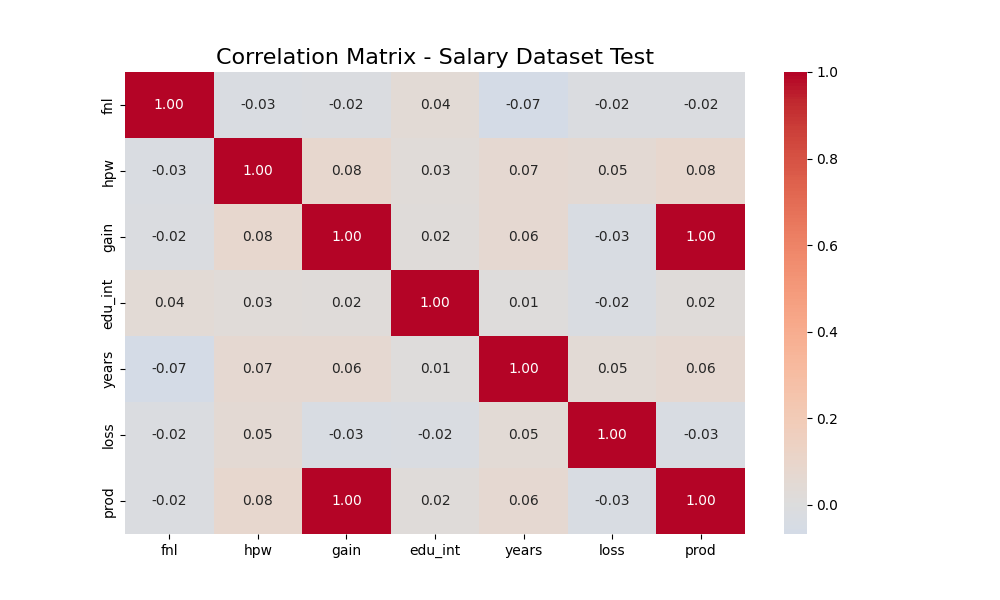
\includegraphics[width=0.8\textwidth]{Resources/matrix_salary_test.png}
    \caption{Correlation Matrix - Numerical Attributes - Salary Dataset Test}
\end{figure}

\newpage
\subsubsection{Categorical Attributes}
\begin{figure}[h!]
    \centering
    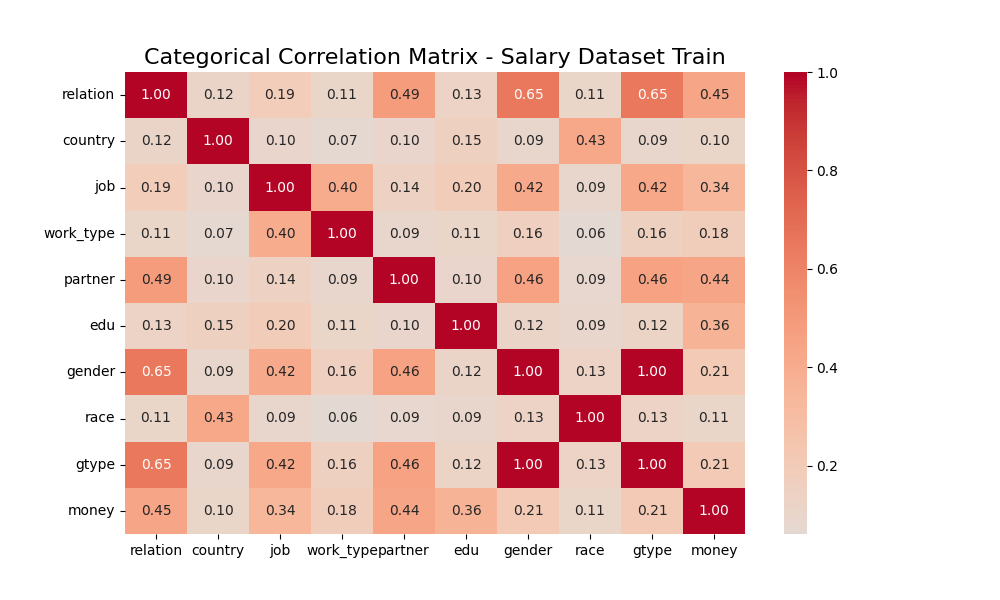
\includegraphics[width=0.8\textwidth]{Resources/matrix_categorial_salary_train.png}
    \caption{Categorical Correlation Matrix - Salary Dataset Train}
\end{figure}

\begin{figure}[h!]
    \centering
    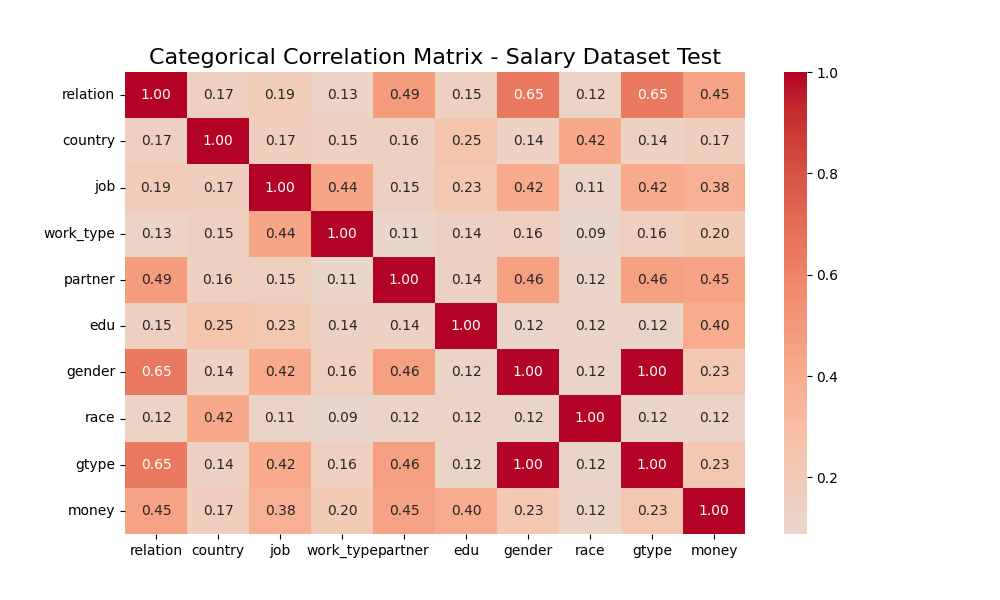
\includegraphics[width=0.8\textwidth]{Resources/matrix_categorial_salary_test.png}
    \caption{Categorical Correlation Matrix - Salary Dataset Test}
\end{figure}

\newpage
\subsection{Comments}
The correlation matrices provide insights into the relationships between different attributes in the datasets.

\subsubsection{AVC Dataset}
\paragraph{Numerical Attributes}
From the numerical attribute correlation matrices of the AVC dataset, it is observed that:
\begin{itemize}
    \item There is a moderate positive correlation between \textit{years\_old} and \textit{biological\_age\_index} in both train and test sets, which indicates that as the age of the person increases, the biological age index also tends to be higher.
    \item \textit{Analysis\_results} show a high correlation with \textit{blood\_sugar\_level}, but low with other numerical attributes, suggesting that the results of medical analyses are relatively independent of the person's age and other indicators.
\end{itemize}

\paragraph{Categorical Attributes}
The categorical correlation matrices for the AVC dataset indicate:
\begin{itemize}
    \item There are some moderate correlations between categorical variables such as \textit{married} and \textit{job\_category}, and \textit{job\_category} and \textit{tobacco\_usage}.
    \item These correlations suggest that there might be certain patterns or dependencies between the demographic and lifestyle attributes.
    \item There is a high correlation between \textit{chaotic\_sleep} and \textit{high\_blood\_pressure}, indicating that individuals with irregular sleep schedules are more likely to have high blood pressure.
\end{itemize}

\subsubsection{Salary Dataset}
\paragraph{Numerical Attributes}
For the Salary dataset, the numerical attribute correlation matrices reveal:
\begin{itemize}
    \item A strong positive correlation between \textit{gain} and \textit{prod}, indicating that individuals who gain more also tend to have higher produce of capital.
    \item \textit{Hours per week (hpw)} shows a low correlation with most other numerical attributes, suggesting that the number of hours worked per week is not strongly related to other numerical factors like capital gains or losses.
\end{itemize}

\paragraph{Categorical Attributes}
In the categorical correlation matrices for the Salary dataset:
\begin{itemize}
    \item Moderate correlations are observed between \textit{work\_type} and \textit{job}, as well as between \textit{country} and \textit{race}.
    \item These correlations highlight possible demographic and professional patterns.
    \item There is also a high correlation between \textit{gtype} and \textit{gender}, indicating that the type of work contract is directly influenced by the gender.
\end{itemize}

Overall, these correlation matrices help in understanding the interdependencies between attributes, which can be useful in feature selection and in improving the performance of machine learning models.

Eliminating specific variables such as \textit{analysis\_results} and \textit{biological\_age\_index} from the AVC dataset, and prod from the Salary dataset, can enhance the efficiency and performance of our machine learning models. These variables were identified as candidates for elimination due to their high correlation with other attributes, which makes them redundant, and their minimal impact on predictive accuracy. By removing these redundant or less impactful features, we reduce noise, prevent overfitting, and simplify the model, leading to improved generalization and more robust predictive performance. This streamlined approach allows the model to focus on the most significant attributes, enhancing both computational efficiency and model interpretability.

\section{Preprocess of Data}

Preprocessing data is a crucial step in machine learning. It involves cleaning, transforming, and encoding data to make it suitable for modeling. Below are the steps and functions used in our preprocessing pipeline.

\subsection{Imputing Missing Values}
Missing values are imputed using the mean for numeric columns and the most frequent value for categorical columns.

\begin{verbatim}
def impute_missing_values(df, nmr_cols, cat_cols, fit, imp):
    df_nmr = df[nmr_cols]
    df_cat = df[cat_cols]
    df.replace('?', np.nan, inplace=True)
    if fit:
        # Fit imputer if on training data
        imp = SimpleImputer(strategy='mean')
        df_nmr_imputed = pd.DataFrame(imp.fit_transform(df_nmr), cols=nmr_cols)
        imp = SimpleImputer(strategy='most_frequent')
        df_cat_imputed = pd.DataFrame(imp.fit_transform(df_cat), cols=cat_cols)
    else:
        # Use the fitted imputer from training data 
        df_nmr_imputed = pd.DataFrame(imp['nmr'].transform(df_nmr), cols=nmr_cols)
        df_cat_imputed = pd.DataFrame(imp['cat'].transform(df_cat), cols=cat_cols)

    df_imputed = pd.concat([df_nmr_imputed, df_cat_imputed], axis=1)
    return df_imputed, imputers
\end{verbatim}

\newpage
\subsection{Handling Extreme Values}
Extreme values are handled using the Interquartile Range (IQR) method and then imputed.

\begin{verbatim}
def handle_extreme_values(df, nmr_cols):
    # Handling extreme values using IQR method
    Q1 = df[nmr_cols].quantile(0.25)
    Q3 = df[nmr_cols].quantile(0.75)
    IQR = Q3 - Q1
    lower_bound = Q1 - 1.5 * IQR
    upper_bound = Q3 + 1.5 * IQR

    # Replace extreme values with NaN
    for col in nmr_cols:
        df[col] = np.where((df[col] < lower_bound[col]) | 
                            (df[col] > upper_bound[col]), 
                            np.nan, df[col])
    
    # Impute missing values for the added NaNs
    imputer = SimpleImputer(strategy='mean')
    df[nmr_cols] = imputer.fit_transform(df[nmr_cols])
    return df
\end{verbatim}

\subsection{Removing Highly Correlated Attributes}
Attributes with high or medium high correlation (above 0.5) are removed to prevent multicollinearity.
Correlation classes:
\newline
-0 to 0.3: low correlation
\newline
-0.3 to 0.7: medium correlation
\newline
-0.7 to 1: high correlation
\newline

This resulted in the following eliminations: \textbf{analysis\_results} and \textbf{biological\_age\_index} from the AVC dataset, and \textbf{prod} from the Salary dataset.
\begin{verbatim}
def remove_redundant_attributes(df, nmr_cols, threshold=0.9):
    numeric_df = df[nmr_cols]

    # Get upper triangle of correlation matrix
    corr_mat = numeric_df.corr().abs()
    upper = corr_mat.where(np.triu(np.ones(corr_mat.shape), k=1).astype(bool))

    # Drop everything higher than threshold
    to_drop = [col for col in upper.cols if any(upper[col] > threshold)]
    df_reduced = df.drop(cols=to_drop)
    return df_reduced, to_drop
\end{verbatim}


\newpage
\subsection{Standardizing Numerical Attributes}
Standardizing ensures that the numerical attributes have a mean of 0 and a standard deviation of 1.

\begin{verbatim}
def standardize_data(df, nmr_cols, method='standard', fit=True, scaler=None):
    if fit:
        if method == 'standard':
            scaler = StandardScaler()
        elif method == 'minmax':
            scaler = MinMaxScaler()
        elif method == 'robust':
            scaler = RobustScaler()
        df[nmr_cols] = scaler.fit_transform(df[nmr_cols])
        return df, scaler
    else:
        df[nmr_cols] = scaler.transform(df[nmr_cols])
        return df
\end{verbatim}

\subsection{Encoding Categorical Variables}
Categorical variables are encoded using OneHotEncoder, and the target variable is encoded using LabelEncoder.

\begin{verbatim}
def encode_categorical(df, trg_col, enc=None):
    df = df.copy()
    cat_cols = df.select_dtypes(include=['object']).cols.tolist()

    # Remove target column from categorical columns
    if trg_col in categorical_cols:
        cat_cols.remove(trg_col)
    
    # Encode target column
    label_enc = LabelEncoder()
    df[trg_col] = label_enc.fit_transform(df[trg_col])
    
    # Encode categorical columns
    enc = OneHotEncoder(sparse_output=False, drop='first', handle_unknown='ignore')
    df_onehot = pd.DataFrame(enc.fit_transform(df[categorical_cols]), 
                             cols=enc.get_feature_names_out(categorical_cols))
    
    df = pd.concat([df, df_onehot], axis=1)
    df.drop(categorical_cols, axis=1, inplace=True)
    
    return df, label_enc, enc
\end{verbatim}

\newpage
\subsection{Wrapper Function for Preprocessing}
The wrapper function applies the above steps to each dataset (training and test) and saves the processed data.

\begin{verbatim}
def preprocess_data_wrapper():
    for name, df in datasets.items():
        if 'train' in name:
            df_reduced, dropped_cols = rm_redundant(..., threshold=0.5)
            nmr_cols_after_drop = [col for col in nmr_cols if col not in dropped]

            df_imputed, imputer = inpute_missing(...)
            fitted_imputers[name] = imputer

            df_outliers_handled = handle_extreme_values(...)

            df_standardized, scaler = standardize_data(...)
            fitted_scalers[name] = scaler

            df_encoded, label_enc, onehot_enc = encode_categorical(...)
            fitted_encs[name] = (label_enc, onehot_enc)

            processed_datasets[name] = df_encoded
        else:
            dropped = [col for col in nmr_cols if col not in proc_df.cols]
            nmr_cols_after_drop = [col for col in nmr_cols if col not in dropped]

            imputer = fitted_imputers[train_name]
            scaler = fitted_scalers[train_name]

            df_imputed, _ = impute_missing_values(...)
            df_outliers_handled = handle_extreme_values(...)
            df_outliers_imputed, _ = impute_missing_values(...)
            df_standardized = standardize_data(...)
            df_encoded, _, _ = encode_categorical(...)

            train_cols = processed_datasets[train_name].cols
            for col in train_cols:
                if col not in df_encoded.cols:
                    df_encoded[col] = 0
            df_encoded = df_encoded[train_cols]

            processed_datasets[name] = df_encoded

    X_avc_train, T_avc_train, _, _ = preprocess_data(...)
    X_avc_test, T_avc_test, _, _ = preprocess_data(...)
    X_salary_train, T_salary_train, _, _ = preprocess_data(...)
    X_salary_test, T_salary_test, _, _ = preprocess_data(...)
    return return_tuple_avc, return_tuple_salary

    def preprocess_data(df, target_column, enc=None):
        # Preprocess the data by encoding cat variables and separating features
        df_enc, label_enc, enc = encode_categorical(df, target_column, enc)
        # Separate features
        X = df_enc.drop(columns=[target_column]).values
        # Separate target
        T = df_enc[target_column].values
        return X, T, label_enc, enc
\end{verbatim}

\section{Logistic Regression}

\subsection{Manual Implementation}
In this section, we implement logistic regression from scratch. The steps involved are as follows:

\begin{itemize}
    \item \textbf{Logistic Function}: Apply the logistic (sigmoid) function to transform input values into probabilities.
    \item \textbf{Negative Log-Likelihood (NLL)}: Compute the NLL, which measures how well the predicted probabilities match the true labels.
    \item \textbf{Accuracy}: Calculate the accuracy of the predictions by comparing them to the true labels.
    \item \textbf{Prediction}: Make predictions using the logistic regression model.
    \item \textbf{Training and Evaluation}: Train the logistic regression model using gradient descent and evaluate its performance.
\end{itemize}

\begin{verbatim}
function logistic(x):
    # Sigmoid function
    return 1 / (1 + exp(-x))

function nll(Y, T):
    # Negative Log-Likelihood
    N = number of samples
    return -sum(T * log(Y) + (1 - T) * log(1 - Y)) / N











function accuracy(Y, T):
    # Accuracy calculation
    N = number of samples
    acc = 0

    # Compare predictions to true labels
    for i in range(N):
        if (Y[i] >= 0.5 and T[i] == 1) or (Y[i] < 0.5 and T[i] == 0):
            acc += 1
    return acc / N

function predict_logistic(X, w):
    # Make predictions using logistic regression model
    return logistic(dot(X, w))

function train_and_eval_logistic(X_train, T_train, X_test, T_test, lr, epochs_no):
    N, D = shape of X_train
    w = random weights
    train_acc, test_acc = []
    train_nll, test_nll = []

    for epoch in range(epochs_no):
        # Make predictions
        Y_train = predict_logistic(X_train, w)
        Y_test = predict_logistic(X_test, w)

        # Calculate metrics
        train_acc.append(accuracy(Y_train, T_train))
        test_acc.append(accuracy(Y_test, T_test))
        train_nll.append(nll(Y_train, T_train))
        test_nll.append(nll(Y_test, T_test))

        # Update weights using gradient descent
        w = w - lr * dot(transpose(X_train), (Y_train - T_train)) / N

    return w, train_nll, test_nll, train_acc, test_acc
\end{verbatim}

\subsection{Scikit-learn Implementation}
In this section, we use the \texttt{scikit-learn} library to implement logistic regression. The steps involved are:

\begin{itemize}
    \item \textbf{Model Initialization}: Initialize the logistic regression model with a maximum of 1000 iterations.
    \item \textbf{Model Fitting}: Fit the model to the training data.
    \item \textbf{Prediction}: Make predictions on the training and test sets.
    \item \textbf{Evaluation}: Calculate accuracy and NLL for the training and test sets.
\end{itemize}


\begin{verbatim}
function train_and_eval_sklearn_logistic(X_train, T_train, X_test, T_test, C, solver):
    # Initialize logistic regression model
    model = LogisticRegression(penalty=penalty, C=C, solver=solver, max_iter=1000)

    # Fit the model
    model.fit(X_train, T_train)

    # Make predictions
    Y_train = model.predict_proba(X_train)[:, 1]
    Y_test = model.predict_proba(X_test)[:, 1]

    # Calculate metrics
    train_acc = accuracy_score(T_train, (Y_train >= 0.5).astype(int))
    test_acc = accuracy_score(T_test, (Y_test >= 0.5).astype(int))
    train_nll = log_loss(T_train, Y_train)
    test_nll = log_loss(T_test, Y_test)

    return model, train_nll, test_nll, train_acc, test_acc
\end{verbatim}

\subsection{Particularities}

In this section, we document the specific approach and settings used for our logistic regression algorithm.

\subsubsection{Categorical Attribute Encoding}
For encoding categorical attributes, we employed the following approach:
\begin{itemize}
    \item \textbf{Label Encoding}: The target variable was encoded using Label Encoding, which converts categorical labels into numerical values.
    \item \textbf{One-Hot Encoding}: Other categorical attributes were encoded using One-Hot Encoding. This method creates binary columns for each category, representing the presence or absence of a specific category in the data.
\end{itemize}

\subsubsection{Optimization Algorithm Settings}
We utilized gradient descent as the optimization algorithm with the following settings:
\begin{itemize}
    \item \textbf{Learning Rate}: A learning rate of 0.3 was chosen to control the step size during the update of the weights. This value was selected based on preliminary experiments to balance convergence speed and stability.
    \item \textbf{Epochs}: The number of epochs was set to 1000 to allow the model to converge to an optimal solution. This value was chosen based on the convergence behavior observed during training.
\end{itemize}
\newpage

\section{MLP}

\subsection{Activation Functions}
The following activation functions are used in our MLP implementation:

\begin{itemize}
    \item \textbf{Sigmoid}: \( \sigma(x) = \frac{1}{1 + e^{-x}} \)
    \item \textbf{ReLU (Rectified Linear Unit)}: \( \text{ReLU}(x) = \max(0, x) \)
    \item \textbf{Tanh}: \( \tanh(x) = \frac{e^x - e^{-x}}{e^x + e^{-x}} \)
    \item \textbf{Leaky ReLU}: \( \text{Leaky ReLU}(x) = \max(\alpha x, x) \)
    \item \textbf{ELU (Exponential Linear Unit)}: \( \text{ELU}(x) = x \) if \( x > 0 \), \( \alpha (e^x - 1) \) if \( x \leq 0 \)
\end{itemize}

\subsection{Manual Implementation}
In this section, we manually implement an MLP with the following components:

\begin{itemize}
    \item \textbf{Activation Functions}: Sigmoid, ReLU, Tanh, Leaky ReLU, and ELU
    \item \textbf{Layers}: Linear layer and Dropout layer
    \item \textbf{Loss Function}: Cross-entropy loss
    \item \textbf{Optimizer}: SGD and Adam optimizers
\end{itemize}

\begin{verbatim}
class Linear:
    def __init__(input_dim, output_dim, l2_reg=0.01):
        Initialize weights and biases

    def forward(x):
        return dot(x, weight) + bias
    def backward(x, dldy):
        Compute gradients for weights and biases

    def update(lr):
        Update weights and biases using gradients

class Dropout:
    def __init__(rate=0.5):
        Set dropout rate

    def forward(x, train=True):
        Apply dropout during training

    def backward(x, dldy):
        Return dldy * mask


class FeedForwardNetwork:
    def __init__(layers):
        Initialize network with layers

    def forward(x, train=True):
        Forward pass through all layers
    def backward(dldy):
        Backward pass through all layers

    def update(*args):
        Update parameters for all layers

function train_and_evaluate_manual_mlp(X_train, T_train, X_test, T_test, 
                                       input_size, hidden_size, output_size,
                                       epochs, learning_rate, l2_reg,
                                       batch_size, optimiser):
    Initialize MLP with Linear, Activation, Dropout layers
    Initialize CrossEntropy loss and optimizer
    for epoch in range(epochs):
        Shuffle and batch data
        for each batch:
            Forward pass
            Compute loss
            Backward pass
            Update parameters
        Evaluate on training and test sets
    return mlp, train_acc_list, test_acc_list, train_loss_list, test_loss_list
\end{verbatim}

\subsection{Scikit-learn Implementation}
In this section, we use the \texttt{scikit-learn} library to implement an MLP. The steps involved are:

\begin{itemize}
    \item \textbf{Model Initialization}: Initialize the MLP classifier with specified parameters.
    \item \textbf{Model Fitting}: Fit the model to the training data.
    \item \textbf{Prediction}: Make predictions on the training and test sets.
    \item \textbf{Evaluation}: Calculate accuracy for the training and test sets.
\end{itemize}

\newpage
\begin{verbatim}
function train_and_evaluate_sklearn_mlp(X_train, T_train, X_test, T_test,
                                        hidden_layer_sizes, max_iter,
                                        learning_rate_init, alpha):
    # Initialize the MLP classifier with the specified parameters
    mlp = MLPClassifier(hidden_layer_sizes=hidden_layer_sizes,
                        max_iter=max_iter, learning_rate_init=learning_rate_init,
                        alpha=alpha, random_state=1)

    # Fit the MLP classifier to the training data
    mlp.fit(X_train, T_train)
    
    # Make predictions on the training and test sets
    train_predictions = mlp.predict(X_train)
    test_predictions = mlp.predict(X_test)
    
    # Compute accuracy for training and test sets
    train_accuracy = accuracy_score(T_train, train_predictions)
    test_accuracy = accuracy_score(T_test, test_predictions)
    
    return train_accuracy, test_accuracy, mlp
\end{verbatim}

Using \texttt{scikit-learn}, we leverage pre-built functions for model training and evaluation, simplifying the implementation process while maintaining performance.

\subsection{Optimizer Usage}
In our MLP implementation, we utilized two different optimizers to update the weights and biases of the network during training: Stochastic Gradient Descent (SGD) and Adaptive Moment Estimation. After extensive testing, we found that the SGD optimizer resulted in better overall performance.

\subsubsection{SGD Optimizer}
The SGD optimizer updates the weights and biases of the linear layers using the gradient of the loss function with respect to each parameter.

\begin{verbatim}
class SGDOptimizer:
    def __init__(self, layers, learning_rate=0.001):
        Initialize learning rate and select linear layers

    def update():
        for each linear layer:
            Update weight using gradient descent
            Update bias using gradient descent
\end{verbatim}

The SGD optimizer provided better results in our experiments, possibly due to its simplicity and effectiveness in handling the specific characteristics of our datasets.

\subsubsection{Adam Optimizer}
The Adam optimizer is an advanced optimization technique that combines the advantages of both the AdaGrad and RMSProp algorithms. It uses adaptive learning rates for each parameter and maintains running averages of the first and second moments of the gradients. The pseudocode for the Adam optimizer is as follows:

\begin{verbatim}
class AdamOptimizer:
    def __init__(self, layers, learning_rate, beta1, beta2, epsilon):
        Initialize parameters and select linear layers

    def update():
        Increment timestep
        for each linear layer:
            Update first moment estimate (m)
            Update second moment estimate (v)
            Compute bias-corrected first moment estimate (m_hat)
            Compute bias-corrected second moment estimate (v_hat)
            Update weight using Adam update rule
            Update bias using Adam update rule
\end{verbatim}

Although the Adam optimizer is generally known for its robust performance across various tasks, in our specific case, the SGD optimizer provided better results. This may be due to the nature of our data and the specific architecture of our MLP, where the more straightforward approach of SGD was more effective.


\subsection{Particularities}

In this section, we document the hyperparameterization and specific configurations used for the Multi-Layer Perceptron (MLP) neural network.

\subsubsection{Architecture}
For the architecture of the MLP, the following configurations were used:
\begin{itemize}
    \item \textbf{Number and Size of Layers}:
    \begin{itemize}
        \item \textbf{AVC Dataset (Manual Implementation)}: 
        \begin{itemize}
            \item Input Layer: Size equal to the number of features in the AVC training set.
            \item Hidden Layer: 100 neurons.
            \item Output Layer: 2 neurons (binary classification).
        \end{itemize}
        \item \textbf{Salary Dataset (Manual Implementation)}: 
        \begin{itemize}
            \item Input Layer: Size equal to the number of features in the Salary training set.
            \item Hidden Layer: 100 neurons.
            \item Output Layer: 2 neurons (binary classification).
        \end{itemize}
        \newpage
        \item \textbf{Scikit-learn Implementation}: 
        \begin{itemize}
            \item Hidden Layers: 100, 50, 25 neurons for each dataset.
        \end{itemize}
    \end{itemize}
    \item \textbf{Activation Functions}:
    \begin{itemize}
        \item ELU (Exponential Linear Unit) was used in the manual implementation proven to be effective in our experiments.
        \item Scikit-learn MLP uses ReLU (Rectified Linear Unit) by default.
    \end{itemize}
\end{itemize}

\subsubsection{Optimizer Configuration}
The optimizer settings were as follows:
\begin{itemize}
    \item \textbf{Type of Optimizer}:
    \begin{itemize}
        \item Manual Implementation: Stochastic Gradient Descent (SGD) for avc, Adaptive Moment Estimation (Adam) for salary.
        \item Scikit-learn Implementation: The default optimizer in scikit-learn MLPClassifier.
    \end{itemize}
    \item \textbf{Learning Rate}:
    \begin{itemize}
        \item Manual Implementation: 0.0001 avc, 0.01 salary.
        \item Scikit-learn Implementation: 0.0001 avc, 0.01 salary.
    \end{itemize}
    \item \textbf{Number of Epochs}: 2000 avc, 1500 salary epochs were used for training.
    \item \textbf{Batch Size}: A batch size of 16/32/64 was used for training.
\end{itemize}

\subsubsection{Regularization Methods}
To prevent overfitting and ensure the model generalizes well, the following regularization methods were applied:
\begin{itemize}
    \item \textbf{Early Stopping}: Tested and proven to result in unpredictable loss variation.
    \item \textbf{L2 Regularization}:
    \begin{itemize}
        \item Manual Implementation: A regularization coefficient (l2\_reg) of 0.001 was used. 
        Weight is set as random.randn(input\_dim, output\_dim) * sqrt(2 / input\_dim)
        \item Scikit-learn Implementation: An alpha value of 0.0001 for L2 regularization was used.
    \end{itemize}
    \item \textbf{Dropout}: A common dropout rate of 0.5 was applied in the manual implementation to prevent overfitting.
\end{itemize}

These configurations were selected to balance model complexity, training efficiency, and generalization performance.

\section{Finding Best Hyperparameters}
In order to achieve optimal performance for the logistic regression and multi-layer perceptron (MLP) models, hyperparameter tuning was performed using GridSearchCV. The following are the best hyperparameters found for each model and dataset.

\subsection{Logistic Regression}
For the logistic regression models, the hyperparameters tuned included the regularization strength (C), the penalty type (L1 or L2), and the solver. The best hyperparameters for the AVC and Salary datasets are as follows:

\paragraph{AVC Dataset}
\begin{itemize}
    \item \textbf{C}: 0.01
    \item \textbf{Class Weight}: None
    \item \textbf{Dual}: False
    \item \textbf{Fit Intercept}: True
    \item \textbf{Intercept Scaling}: 1
    \item \textbf{L1 Ratio}: None
    \item \textbf{Max Iterations}: 100
    \item \textbf{Multi Class}: Auto
    \item \textbf{Penalty}: L1
    \item \textbf{Solver}: Liblinear
    \item \textbf{Tolerance}: 0.0001
    \item \textbf{Warm Start}: False
\end{itemize}

\paragraph{Salary Dataset}
\begin{itemize}
    \item \textbf{C}: 10
    \item \textbf{Class Weight}: None
    \item \textbf{Dual}: False
    \item \textbf{Fit Intercept}: True
    \item \textbf{Intercept Scaling}: 1
    \item \textbf{L1 Ratio}: None
    \item \textbf{Max Iterations}: 100
    \item \textbf{Multi Class}: Auto
    \item \textbf{Penalty}: L2
    \item \textbf{Solver}: Liblinear
    \item \textbf{Tolerance}: 0.0001
    \item \textbf{Warm Start}: False
\end{itemize}

\subsection{Multi-Layer Perceptron (MLP)}
For the MLP models, the hyperparameters tuned included the activation function, alpha (L2 penalty), batch size, learning rate initialization, and the solver among others. The best hyperparameters for the AVC and Salary datasets are as follows:

\paragraph{AVC Dataset}
\begin{itemize}
    \item \textbf{Activation}: ReLU
    \item \textbf{Alpha}: 0.0001
    \item \textbf{Batch Size}: Auto
    \item \textbf{Beta\_1}: 0.9
    \item \textbf{Beta\_2}: 0.999
    \item \textbf{Early Stopping}: True
    \item \textbf{Epsilon}: 1e-08
    \item \textbf{Hidden Layer Sizes}: (100, 50, 25)
    \item \textbf{Learning Rate}: Constant
    \item \textbf{Learning Rate Init}: 0.0001
    \item \textbf{Max Fun}: 15000
    \item \textbf{Max Iterations}: 2000
    \item \textbf{Momentum}: 0.9
    \item \textbf{N\_Iter\_No\_Change}: 10
    \item \textbf{Nesterovs Momentum}: True
    \item \textbf{Power\_T}: 0.5
    \item \textbf{Shuffle}: True
    \item \textbf{Solver}: SGD
    \item \textbf{Tolerance}: 0.0001
    \item \textbf{Validation Fraction}: 0.1
    \item \textbf{Verbose}: False
    \item \textbf{Warm Start}: False
\end{itemize}

\paragraph{Salary Dataset}
\begin{itemize}
    \item \textbf{Activation}: ReLU
    \item \textbf{Alpha}: 0.01
    \item \textbf{Batch Size}: Auto
    \item \textbf{Beta\_1}: 0.9
    \item \textbf{Beta\_2}: 0.999
    \item \textbf{Early Stopping}: True
    \item \textbf{Epsilon}: 1e-08
    \item \textbf{Hidden Layer Sizes}: (100, 50, 25)
    \item \textbf{Learning Rate}: Constant
    \item \textbf{Learning Rate Init}: 0.001
    \item \textbf{Max Fun}: 15000
    \item \textbf{Max Iterations}: 1500
    \item \textbf{Momentum}: 0.9
    \item \textbf{N\_Iter\_No\_Change}: 10
    \item \textbf{Nesterovs Momentum}: True
    \item \textbf{Power\_T}: 0.5
    \item \textbf{Shuffle}: True
    \item \textbf{Solver}: Adam
    \item \textbf{Tolerance}: 0.0001
    \item \textbf{Validation Fraction}: 0.1
    \item \textbf{Verbose}: False
    \item \textbf{Warm Start}: False
\end{itemize}

\newpage

\section{Comparison}

\subsection{Context}
When comparing different models, it's crucial to consider various evaluation metrics to understand their performance. For binary classification tasks, commonly used metrics include precision, recall, and F1 score. These metrics are defined as follows:

\begin{itemize}
    \item \textbf{Accuracy}: This measures the proportion of true results (both true positives and true negatives) among the total number of cases examined. It is a common metric for evaluating classification models.
    \[
    \text{Accuracy} = \frac{TP + TN}{TP + TN + FP + FN}
    \]
    where \( TP \) is the number of true positives, \( TN \) is the number of true negatives, \( FP \) is the number of false positives, and \( FN \) is the number of false negatives.

    \item \textbf{Macro Average (Macro Avg)}: This is the average of the precision, recall, and F1-score calculated for each class separately. It treats all classes equally, regardless of their support (number of samples).
    \[
    \text{Macro Precision} = \frac{\text{Precision}_0 + \text{Precision}_1}{2}
    \]
    \[
    \text{Macro Recall} = \frac{\text{Recall}_0 + \text{Recall}_1}{2}
    \]
    \[
    \text{Macro F1} = \frac{\text{F1 Score}_0 + \text{F1 Score}_1}{2}
    \]

    \item \textbf{Weighted Average (Weighted Avg)}: This is the average of the precision, recall, and F1-score calculated for each class, weighted by the number of true instances for each class. It accounts for class imbalance by giving more weight to classes with more instances.
    \[
    \text{Weighted Precision} = \frac{\text{Precision}_0 \times \text{Support}_0 + \text{Precision}_1 \times \text{Support}_1}{\text{Support}_0 + \text{Support}_1}
    \]
    \[
    \text{Weighted Recall} = \frac{\text{Recall}_0 \times \text{Support}_0 + \text{Recall}_1 \times \text{Support}_1}{\text{Support}_0 + \text{Support}_1}
    \]
    \[
    \text{Weighted F1} = \frac{\text{F1 Score}_0 \times \text{Support}_0 + \text{F1 Score}_1 \times \text{Support}_1}{\text{Support}_0 + \text{Support}_1}
    \]

    \item \textbf{Precision}: The ratio of true positive predictions to the total number of positive predictions made by the model. It indicates the accuracy of the positive predictions.
    \[
    \text{Precision} = \frac{TP}{TP + FP}
    \]

    \item \textbf{Recall}: The ratio of true positive predictions to the total number of actual positive instances. It measures the model's ability to capture all positive instances.
    \[
    \text{Recall} = \frac{TP}{TP + FN}
    \]

    \item \textbf{F1 Score}: The harmonic mean of precision and recall. It provides a balance between precision and recall and is especially useful when the class distribution is imbalanced.
    \[
    \text{F1 Score} = 2 \times \frac{\text{Precision} \times \text{Recall}}{\text{Precision} + \text{Recall}}
    \]
\end{itemize}

These metrics provide a comprehensive view of the model's performance, ensuring that both the accuracy of positive predictions and the ability to capture all positive instances are considered. When dealing with imbalanced datasets, the F1 score becomes particularly important as it balances the trade-off between precision and recall.

\subsection{Logistic Regression Performance}

\subsubsection{AVC Dataset Metrics}

\begin{table}[h!]
    \centering
    \caption{Manual LogReg - AVC LogReg Train}
    \begin{tabularx}{\textwidth}{|l|X|X|X|X|}
    \hline
    \textbf{Metric} & \textbf{Precision} & \textbf{Recall} & \textbf{F1-Score} & \textbf{Support} \\
    \hline
    Class 0 & 0.957608 & 0.998467 & 0.977611 & 3914 \\
    Class 1 & 0.142857 & 0.005747 & 0.011050 & 174 \\
    Accuracy & 0.956213 & 0.956213 & 0.956213 & 0.956213 \\
    Macro Avg & 0.550233 & 0.502107 & 0.494330 & 4088 \\
    Weighted Avg & 0.922930 & 0.956213 & 0.936471 & 4088 \\
    \hline
    \end{tabularx}
    \end{table}
    
    \begin{table}[h!]
    \centering
    \caption{Manual LogReg - AVC LogReg Test}
    \begin{tabularx}{\textwidth}{|l|X|X|X|X|}
    \hline
    \textbf{Metric} & \textbf{Precision} & \textbf{Recall} & \textbf{F1-Score} & \textbf{Support} \\
    \hline
    Class 0 & 0.928361 & 0.998944 & 0.962360 & 947 \\
    Class 1 & 0.666667 & 0.026667 & 0.051282 & 75 \\
    Accuracy & 0.927593 & 0.927593 & 0.927593 & 0.927593 \\
    Macro Avg & 0.797514 & 0.512805 & 0.506821 & 1022 \\
    Weighted Avg & 0.909157 & 0.927593 & 0.895500 & 1022 \\
    \hline
    \end{tabularx}
    \end{table}
    
    \begin{table}[h!]
    \centering
    \caption{Scikit-learn LogReg - AVC LogReg Train}
    \begin{tabularx}{\textwidth}{|l|X|X|X|X|}
    \hline
    \textbf{Metric} & \textbf{Precision} & \textbf{Recall} & \textbf{F1-Score} & \textbf{Support} \\
    \hline
    Class 0 & 0.957436 & 1.000000 & 0.978255 & 3914 \\
    Class 1 & 0.000000 & 0.000000 & 0.000000 & 174 \\
    Accuracy & 0.957436 & 0.957436 & 0.957436 & 0.957436 \\
    Macro Avg & 0.478718 & 0.500000 & 0.489128 & 4088 \\
    Weighted Avg & 0.916684 & 0.957436 & 0.936617 & 4088 \\
    \hline
    \end{tabularx}
    \end{table}
    
    \begin{table}[h!]
    \centering
    \caption{Scikit-learn LogReg - AVC LogReg Test}
    \begin{tabularx}{\textwidth}{|l|X|X|X|X|}
    \hline
    \textbf{Metric} & \textbf{Precision} & \textbf{Recall} & \textbf{F1-Score} & \textbf{Support} \\
    \hline
    Class 0 & 0.926614 & 1.000000 & 0.961910 & 947 \\
    Class 1 & 0.000000 & 0.000000 & 0.000000 & 75 \\
    Accuracy & 0.926614 & 0.926614 & 0.926614 & 0.926614 \\
    Macro Avg & 0.463307 & 0.500000 & 0.480955 & 1022 \\
    Weighted Avg & 0.858614 & 0.926614 & 0.891319 & 1022 \\
    \hline
    \end{tabularx}
    \end{table}
    
    \newpage
\subsubsection{Salary Dataset Metrics}
    
    \begin{table}[h!]
    \centering
    \caption{Manual LogReg - Salary LogReg Train}
    \begin{tabularx}{\textwidth}{|l|X|X|X|X|}
    \hline
    \textbf{Metric} & \textbf{Precision} & \textbf{Recall} & \textbf{F1-Score} & \textbf{Support} \\
    \hline
    Class 0 & 0.858587 & 0.922014 & 0.889171 & 6078 \\
    Class 1 & 0.677989 & 0.519521 & 0.588270 & 1921 \\
    Accuracy & 0.825353 & 0.825353 & 0.825353 & 0.825353 \\
    Macro Avg & 0.768288 & 0.720767 & 0.738720 & 7999 \\
    Weighted Avg & 0.815216 & 0.825353 & 0.816908 & 7999 \\
    \hline
    \end{tabularx}
    \end{table}
    
    \begin{table}[h!]
    \centering
    \caption{Manual LogReg - Salary LogReg Test}
    \begin{tabularx}{\textwidth}{|l|X|X|X|X|}
    \hline
    \textbf{Metric} & \textbf{Precision} & \textbf{Recall} & \textbf{F1-Score} & \textbf{Support} \\
    \hline
    Class 0 & 0.854957 & 0.923331 & 0.887830 & 1513 \\
    Class 1 & 0.683060 & 0.513347 & 0.586166 & 487 \\
    Accuracy & 0.823500 & 0.823500 & 0.823500 & 0.823500 \\
    Macro Avg & 0.769009 & 0.718339 & 0.736998 & 2000 \\
    Weighted Avg & 0.813100 & 0.823500 & 0.814375 & 2000 \\
    \hline
    \end{tabularx}
    \end{table}
    
    \begin{table}[h!]
    \centering
    \caption{Scikit-learn LogReg - Salary LogReg Train}
    \begin{tabularx}{\textwidth}{|l|X|X|X|X|}
    \hline
    \textbf{Metric} & \textbf{Precision} & \textbf{Recall} & \textbf{F1-Score} & \textbf{Support} \\
    \hline
    Class 0 & 0.869088 & 0.925140 & 0.896238 & 6078 \\
    Class 1 & 0.702420 & 0.559084 & 0.622609 & 1921 \\
    Accuracy & 0.837230 & 0.837230 & 0.837230 & 0.837230 \\
    Macro Avg & 0.785754 & 0.742112 & 0.759424 & 7999 \\
    Weighted Avg & 0.829062 & 0.837230 & 0.830525 & 7999 \\
    \hline
    \end{tabularx}
    \end{table}
    
    \begin{table}[h!]
    \centering
    \caption{Scikit-learn LogReg - Salary LogReg Test}
    \begin{tabularx}{\textwidth}{|l|X|X|X|X|}
    \hline
    \textbf{Metric} & \textbf{Precision} & \textbf{Recall} & \textbf{F1-Score} & \textbf{Support} \\
    \hline
    Class 0 & 0.863748 & 0.925975 & 0.893780 & 1513 \\
    Class 1 & 0.703704 & 0.546201 & 0.615029 & 487 \\
    Accuracy & 0.833500 & 0.833500 & 0.833500 & 0.833500 \\
    Macro Avg & 0.783726 & 0.736088 & 0.754404 & 2000 \\
    Weighted Avg & 0.824778 & 0.833500 & 0.825904 & 2000 \\
    \hline
    \end{tabularx}
    \end{table}
\newpage

\subsubsection{Observations}
\begin{itemize}
    \item \textbf{AVC Dataset:} Both manual and scikit-learn logistic regression models perform similarly in terms of precision, recall, and F1-score for Class 0. However, the manual implementation shows slightly higher test accuracy.
    \item \textbf{Salary Dataset:} The scikit-learn implementation shows a marginal improvement in both train and test accuracy compared to the manual implementation. Precision, recall, and F1-score for Class 0 are also slightly higher in the scikit-learn implementation.
\end{itemize}

Overall, while both implementations provide comparable results, the scikit-learn implementation offers slightly better performance metrics in the Salary dataset and marginally higher train accuracy in the AVC dataset.

\subsubsection{Confusion Matrices}

\begin{figure}[H]
    \centering
    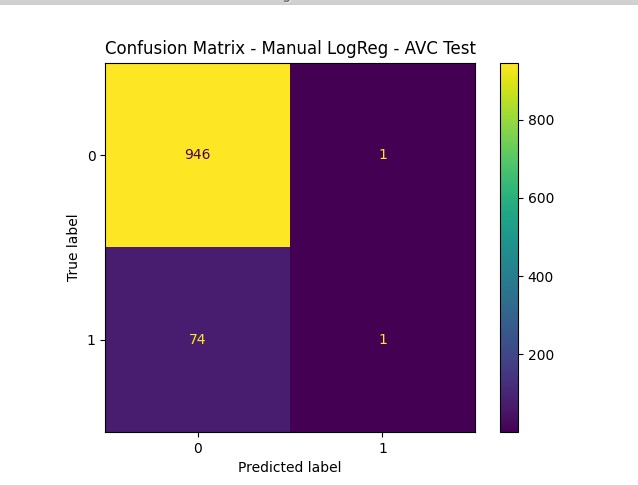
\includegraphics[width=0.45\textwidth]{Resources/logreg_manual_confusion_avc_test.jpeg}
    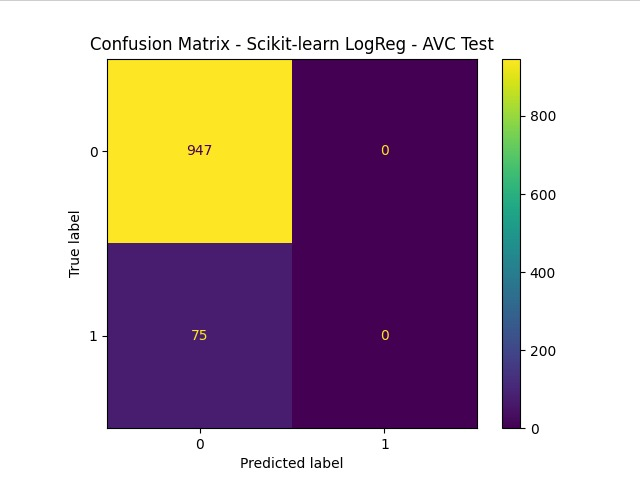
\includegraphics[width=0.45\textwidth]{Resources/logreg_scikit_confusion_avc_test.jpeg}
    \caption{Confusion Matrices for AVC Dataset - Test Set}
    \label{fig:confusion_avc_test}
\end{figure}

\begin{figure}[H]
    \centering
    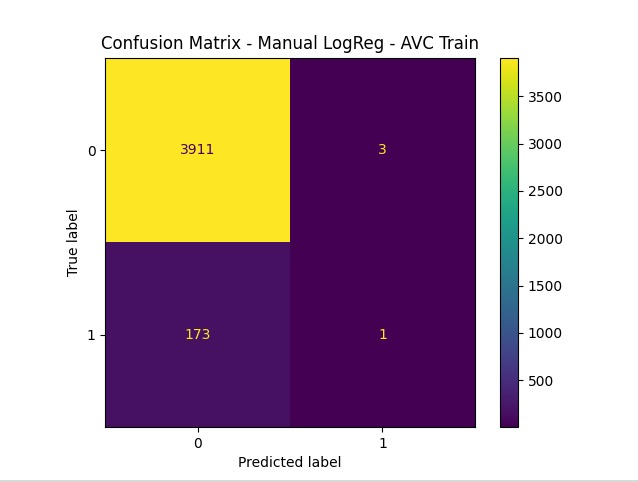
\includegraphics[width=0.45\textwidth]{Resources/logreg_manual_confusion_avc_train.jpeg}
    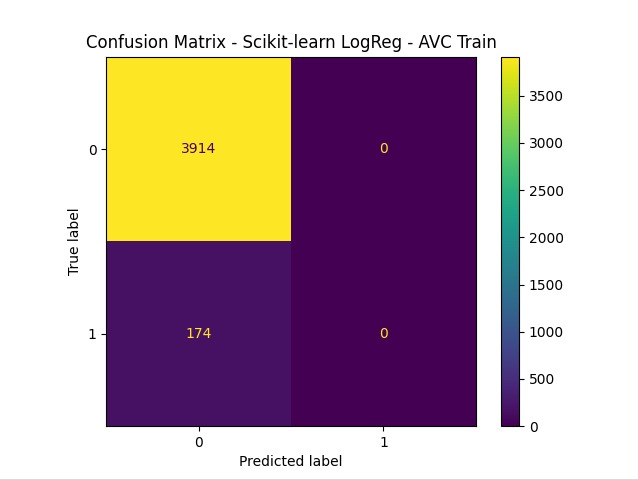
\includegraphics[width=0.45\textwidth]{Resources/logreg_scikit_confusion_avc_train.jpeg}
    \caption{Confusion Matrices for AVC Dataset - Train Set}
    \label{fig:confusion_avc_train}
\end{figure}

\begin{figure}[H]
    \centering
    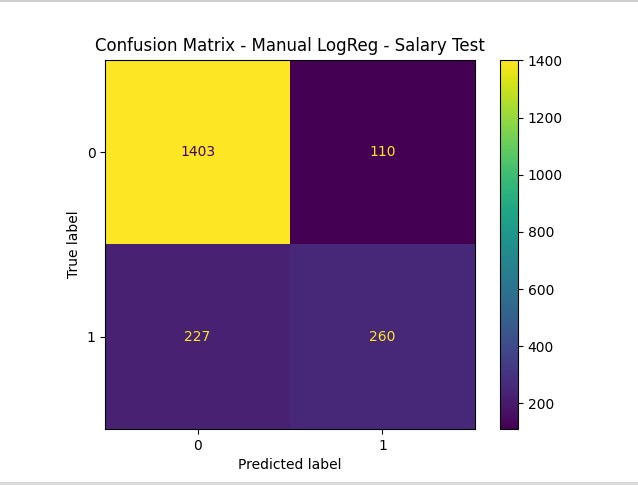
\includegraphics[width=0.45\textwidth]{Resources/logreg_manual_confusion_salary_test.jpeg}
    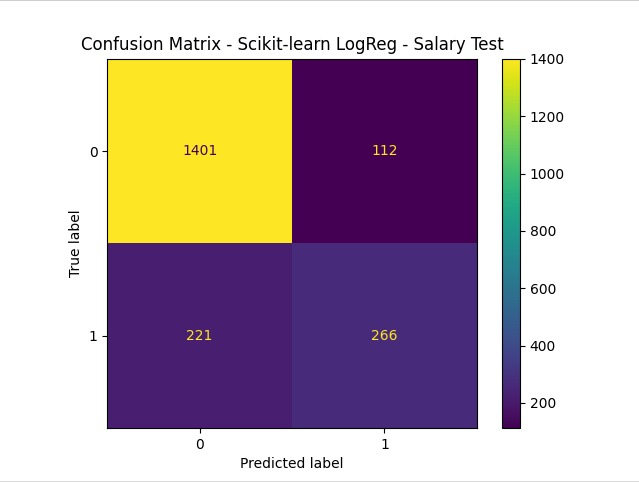
\includegraphics[width=0.45\textwidth]{Resources/logreg_scikit_confusion_salary_test.jpeg}
    \caption{Confusion Matrices for Salary Dataset - Test Set}
    \label{fig:confusion_salary_test}
\end{figure}

\begin{figure}[H]
    \centering
    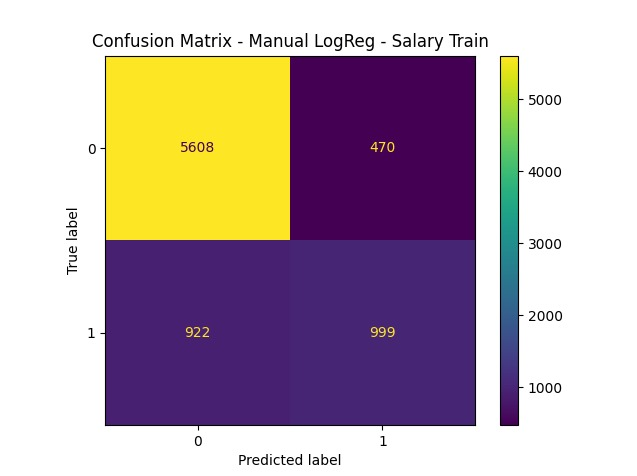
\includegraphics[width=0.45\textwidth]{Resources/logreg_manual_confusion_salary_train.jpeg}
    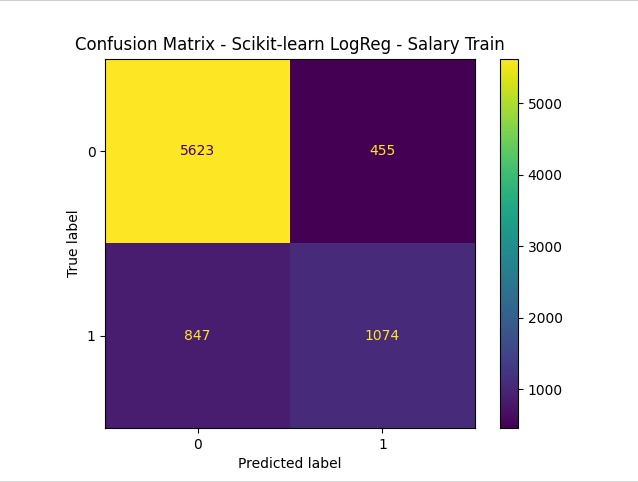
\includegraphics[width=0.45\textwidth]{Resources/logreg_scikit_confusion_salary_train.jpeg}
    \caption{Confusion Matrices for Salary Dataset - Train Set}
    \label{fig:confusion_salary_train}
\end{figure}

\subsubsection{Comments on Confusion Matrices}

\paragraph{AVC Dataset - Test Set}
\begin{itemize}
    \item \textbf{Manual Logistic Regression}:
    \begin{itemize}
        \item Correctly predicted majority of the negative class (946 out of 947).
        \item Struggled with the positive class, only predicting 1 out of 75 correctly.
        \item This results in high accuracy for the negative class but very low recall for the positive class, indicating the model's inability to correctly identify positive cases.
    \end{itemize}
    \item \textbf{Scikit-learn Logistic Regression}:
    \begin{itemize}
        \item Correctly predicted all negative cases (947 out of 947).
        \item Failed to predict any positive cases (0 out of 75).
        \item Similar to the manual implementation, this model has high precision and recall for the negative class but fails to identify any positive instances.
    \end{itemize}
\end{itemize}

\paragraph{AVC Dataset - Train Set}
\begin{itemize}
    \item \textbf{Manual Logistic Regression}:
    \begin{itemize}
        \item Correctly predicted almost all negative cases (3911 out of 3914).
        \item Only a small number of positive cases predicted correctly (1 out of 174).
        \item Shows overfitting to the negative class with high accuracy for the negative class and low performance for the positive class.
    \end{itemize}
    \item \textbf{Scikit-learn Logistic Regression}:
    \begin{itemize}
        \item Predicted all negative cases correctly (3914 out of 3914).
        \item Like the manual implementation, failed to predict any positive cases (0 out of 174).
        \item Indicates overfitting to the negative class, similar to the test set performance.
    \end{itemize}
\end{itemize}

\paragraph{Salary Dataset - Test Set}
\begin{itemize}
    \item \textbf{Manual Logistic Regression}:
    \begin{itemize}
        \item Predicted majority of the negative class correctly (1403 out of 1513).
        \item Managed to identify a significant portion of the positive class (260 out of 487).
        \item Shows a better balance compared to the AVC dataset, with reasonable performance on both classes.
    \end{itemize}
    \item \textbf{Scikit-learn Logistic Regression}:
    \begin{itemize}
        \item Similar performance to the manual implementation for the negative class (1401 out of 1513).
        \item Slightly better performance for the positive class (266 out of 487).
        \item This indicates a well-balanced model for both classes, showing better generalization.
    \end{itemize}
\end{itemize}

\paragraph{Salary Dataset - Train Set}
\begin{itemize}
    \item \textbf{Manual Logistic Regression}:
    \begin{itemize}
        \item Correctly predicted majority of the negative class (5608 out of 6078).
        \item Identified a substantial number of positive cases (989 out of 1921).
        \item This model shows good generalization with balanced performance across both classes.
    \end{itemize}
    \item \textbf{Scikit-learn Logistic Regression}:
    \begin{itemize}
        \item High accuracy for the negative class (5623 out of 6078).
        \item Good performance for the positive class as well (1074 out of 1921).
        \item Indicates the model's robustness and ability to generalize well to both classes.
    \end{itemize}
\end{itemize}

\paragraph{Summary}
\begin{itemize}
    \item The confusion matrices for the AVC dataset show a significant bias towards the negative class, with both manual and scikit-learn logistic regression models struggling to predict positive cases.
    \item For the Salary dataset, both models exhibit a more balanced performance, accurately predicting both negative and positive cases, though scikit-learn logistic regression performs slightly better on the test set.
    \item This analysis highlights the importance of evaluating model performance across different classes and not solely relying on accuracy as a metric.
\end{itemize}

\subsubsection{Overall Accuracy}

The overall accuracy for the manual and scikit-learn implementations of logistic regression for both datasets (AVC and Salary) is presented below. The accuracy curves are also included to visualize the performance of the models over the epochs.

\begin{figure}[H]
    \centering
    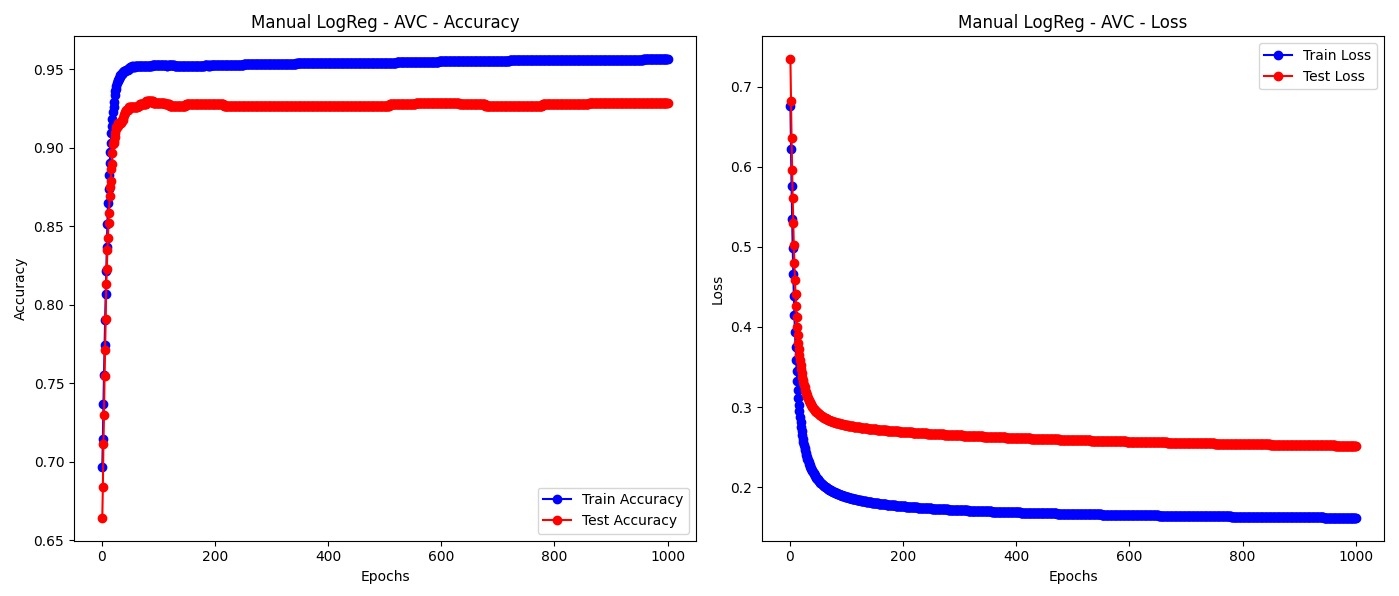
\includegraphics[width=0.9\textwidth]{Resources/logreg_curve_avc.jpeg}
    \caption{Accuracy Curve for Manual Logistic Regression - AVC Dataset}
    \label{fig:logreg_curve_avc}
\end{figure}

\begin{figure}[H]
    \centering
    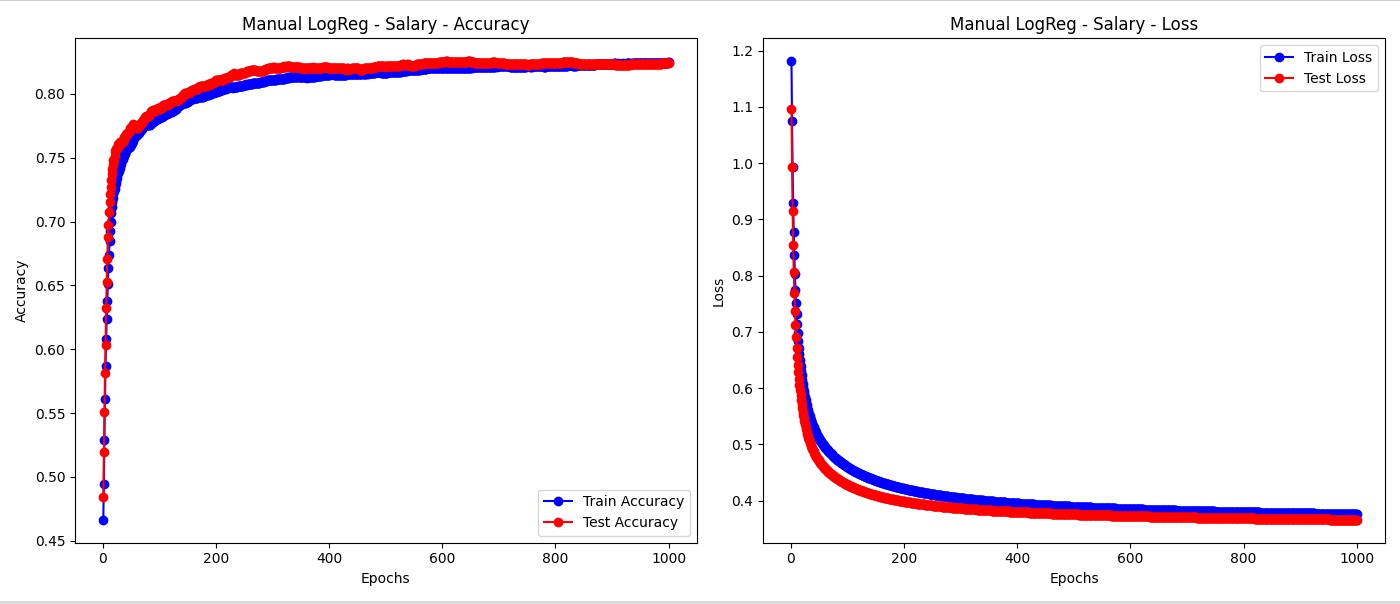
\includegraphics[width=0.9\textwidth]{Resources/logreg_curve_salary.jpeg}
    \caption{Accuracy Curve for Manual Logistic Regression - Salary Dataset}
    \label{fig:logreg_curve_salary}
\end{figure}

The results are summarized as follows:

\textbf{Manual Logistic Regression Results:}
\begin{itemize}
    \item \textbf{AVC Dataset:}
        \begin{itemize}
            \item Train Accuracy: 0.9559686888454012
            \item Test Accuracy: 0.9285714285714286
        \end{itemize}
    \item \textbf{Salary Dataset:}
        \begin{itemize}
            \item Train Accuracy: 0.8241030128766096
            \item Test Accuracy: 0.8215
        \end{itemize}
\end{itemize}

\textbf{Scikit-learn Logistic Regression Results:}
\begin{itemize}
    \item \textbf{AVC Dataset:}
        \begin{itemize}
            \item Train Accuracy: 0.9574363992172211
            \item Test Accuracy: 0.9266144814090019
        \end{itemize}
    \item \textbf{Salary Dataset:}
        \begin{itemize}
            \item Train Accuracy: 0.8372296537067133
            \item Test Accuracy: 0.8335
        \end{itemize}
\end{itemize}

\subsubsection{Overfit Analysis}

\textbf{Manual Logistic Regression - AVC Dataset:}
\begin{itemize}
    \item The train accuracy (0.9559686888454012) is slightly higher than the test accuracy (0.9285714285714286).
    \item The difference between train and test accuracy is around 0.03, which is relatively small, indicating that there is no significant overfitting.
\end{itemize}

\newpage
\textbf{Scikit-learn Logistic Regression - AVC Dataset:}
\begin{itemize}
    \item The train accuracy (0.9574363992172211) is slightly higher than the test accuracy (0.9266144814090019).
    \item The difference between train and test accuracy is around 0.03, similar to the manual implementation, suggesting no significant overfitting.
\end{itemize}

\textbf{Manual Logistic Regression - Salary Dataset:}
\begin{itemize}
    \item The train accuracy (0.8241030128766096) is very close to the test accuracy (0.8215).
    \item The minimal difference indicates that the model generalizes well to the test data, showing no signs of overfitting.
\end{itemize}

\textbf{Scikit-learn Logistic Regression - Salary Dataset:}
\begin{itemize}
    \item The train accuracy (0.8372296537067133) is slightly higher than the test accuracy (0.8335).
    \item The difference is around 0.004, which is very small, indicating no significant overfitting.
\end{itemize}


\subsection{Multi Layer Perceptron}

\subsubsection{AVC Dataset Metrics}

\begin{table}[h!]
    \centering
    \caption{Manual MLP - AVC MLP Train}
    \begin{tabularx}{\textwidth}{|l|X|X|X|X|}
    \hline
    \textbf{Metric} & \textbf{Precision} & \textbf{Recall} & \textbf{F1-Score} & \textbf{Support} \\
    \hline
    Class 0 & 0.957436 & 1.000000 & 0.978255 & 3914 \\
    Class 1 & 0.000000 & 0.000000 & 0.000000 & 174 \\
    Accuracy & 0.957436 & 0.957436 & 0.957436 & 0.957436 \\
    Macro Avg & 0.478718 & 0.500000 & 0.489128 & 4088 \\
    Weighted Avg & 0.916684 & 0.957436 & 0.936617 & 4088 \\
    \hline
    \end{tabularx}
\end{table}

\begin{table}[h!]
    \centering
    \caption{Manual MLP - AVC MLP Test}
    \begin{tabularx}{\textwidth}{|l|X|X|X|X|}
    \hline
    \textbf{Metric} & \textbf{Precision} & \textbf{Recall} & \textbf{F1-Score} & \textbf{Support} \\
    \hline
    Class 0 & 0.926614 & 1.000000 & 0.961910 & 947 \\
    Class 1 & 0.000000 & 0.000000 & 0.000000 & 75 \\
    Accuracy & 0.926614 & 0.926614 & 0.926614 & 0.926614 \\
    Macro Avg & 0.463307 & 0.500000 & 0.480955 & 1022 \\
    Weighted Avg & 0.858614 & 0.926614 & 0.891319 & 1022 \\
    \hline
    \end{tabularx}
\end{table}

\begin{table}[h!]
    \centering
    \caption{Scikit-learn MLP - AVC MLP Train}
    \begin{tabularx}{\textwidth}{|l|X|X|X|X|}
    \hline
    \textbf{Metric} & \textbf{Precision} & \textbf{Recall} & \textbf{F1-Score} & \textbf{Support} \\
    \hline
    Class 0 & 0.997195 & 0.998978 & 0.998086 & 3914 \\
    Class 1 & 0.976048 & 0.936782 & 0.956012 & 174 \\
    Accuracy & 0.996331 & 0.996331 & 0.996331 & 0.996331 \\
    Macro Avg & 0.986621 & 0.967880 & 0.977049 & 4088 \\
    Weighted Avg & 0.996295 & 0.996331 & 0.996295 & 4088 \\
    \hline
    \end{tabularx}
\end{table}

\begin{table}[h!]
    \centering
    \caption{Scikit-learn MLP - AVC MLP Test}
    \begin{tabularx}{\textwidth}{|l|X|X|X|X|}
    \hline
    \textbf{Metric} & \textbf{Precision} & \textbf{Recall} & \textbf{F1-Score} & \textbf{Support} \\
    \hline
    Class 0 & 0.925926 & 0.976769 & 0.950668 & 947 \\
    Class 1 & 0.043478 & 0.013333 & 0.020408 & 75 \\
    Accuracy & 0.906067 & 0.906067 & 0.906067 & 0.906067 \\
    Macro Avg & 0.484702 & 0.495051 & 0.485538 & 1022 \\
    Weighted Avg & 0.861167 & 0.906067 & 0.882400 & 1022 \\
    \hline
    \end{tabularx}
\end{table}

\newpage
\subsubsection{Salary Dataset Metrics}

\begin{table}[h!]
    \centering
    \caption{Manual MLP - Salary MLP Train}
    \begin{tabularx}{\textwidth}{|l|X|X|X|X|}
    \hline
    \textbf{Metric} & \textbf{Precision} & \textbf{Recall} & \textbf{F1-Score} & \textbf{Support} \\
    \hline
    Class 0 & 0.862637 & 0.929911 & 0.895012 & 6078 \\
    Class 1 & 0.705598 & 0.531494 & 0.606295 & 1921 \\
    Accuracy & 0.834229 & 0.834229 & 0.834229 & 0.834229 \\
    Macro Avg & 0.784118 & 0.730703 & 0.750653 & 7999 \\
    Weighted Avg & 0.824924 & 0.834229 & 0.825675 & 7999 \\
    \hline
    \end{tabularx}
\end{table}

\begin{table}[h!]
    \centering
    \caption{Manual MLP - Salary MLP Test}
    \begin{tabularx}{\textwidth}{|l|X|X|X|X|}
    \hline
    \textbf{Metric} & \textbf{Precision} & \textbf{Recall} & \textbf{F1-Score} & \textbf{Support} \\
    \hline
    Class 0 & 0.858788 & 0.936550 & 0.895985 & 1513 \\
    Class 1 & 0.725714 & 0.521561 & 0.606930 & 487 \\
    Accuracy & 0.835500 & 0.835500 & 0.835500 & 0.835500 \\
    Macro Avg & 0.792251 & 0.729055 & 0.751457 & 2000 \\
    Weighted Avg & 0.826384 & 0.835500 & 0.825600 & 2000 \\
    \hline
    \end{tabularx}
\end{table}

\begin{table}[h!]
    \centering
    \caption{Scikit-learn MLP - Salary MLP Train}
    \begin{tabularx}{\textwidth}{|l|X|X|X|X|}
    \hline
    \textbf{Metric} & \textbf{Precision} & \textbf{Recall} & \textbf{F1-Score} & \textbf{Support} \\
    \hline
    Class 0 & 0.978297 & 0.978940 & 0.978618 & 6078 \\
    Class 1 & 0.933229 & 0.931286 & 0.932256 & 1921 \\
    Accuracy & 0.967496 & 0.967496 & 0.967496 & 0.967496 \\
    Macro Avg & 0.955763 & 0.955113 & 0.955437 & 7999 \\
    Weighted Avg & 0.967473 & 0.967496 & 0.967484 & 7999 \\
    \hline
    \end{tabularx}
\end{table}

\begin{table}[h!]
    \centering
    \caption{Scikit-learn MLP - Salary MLP Test}
    \begin{tabularx}{\textwidth}{|l|X|X|X|X|}
    \hline
    \textbf{Metric} & \textbf{Precision} & \textbf{Recall} & \textbf{F1-Score} & \textbf{Support} \\
    \hline
    Class 0 & 0.869479 & 0.871778 & 0.870627 & 1513 \\
    Class 1 & 0.598344 & 0.593429 & 0.595876 & 487 \\
    Accuracy & 0.804000 & 0.804000 & 0.804000 & 0.804000 \\
    Macro Avg & 0.733911 & 0.732604 & 0.733252 & 2000 \\
    Weighted Avg & 0.803458 & 0.804000 & 0.803725 & 2000 \\
    \hline
    \end{tabularx}
\end{table}

\newpage
\subsubsection{Observations}
\begin{itemize}
    \item \textbf{AVC Dataset:} 
    \begin{itemize}
        \item Manual MLP: High precision and recall for Class 0 but poor performance for Class 1, indicating an inability to correctly identify positive cases.
        \item Scikit-learn MLP: Excellent precision and recall for both classes in the training set but struggles with Class 1 in the test set, indicating potential overfitting.
    \end{itemize}
    \item \textbf{Salary Dataset:} 
    \begin{itemize}
        \item Manual MLP: Balanced performance across both classes with decent precision, recall, and F1-scores.
        \item Scikit-learn MLP: Superior performance in the training set with high precision and recall for both classes, but slightly lower generalization in the test set.
    \end{itemize}
\end{itemize}

Overall, while both implementations show good performance, the scikit-learn implementation tends to overfit in the training set but provides better precision and recall in the test set compared to the manual implementation.

\subsubsection{Confusion Matrices}

\begin{figure}[H]
    \centering
    \includegraphics[width=0.45\textwidth]{Resources/mlp_manual_confusion_avc_test.jpeg}
    \includegraphics[width=0.45\textwidth]{Resources/mlp_scikit_confusion_avc_test.jpeg}
    \caption{Confusion Matrices for AVC Dataset - Test Set}
    \label{fig:mlp_confusion_avc_test}
\end{figure}

\begin{figure}[H]
    \centering
    \includegraphics[width=0.45\textwidth]{Resources/mlp_manual_confusion_avc_train.jpeg}
    \includegraphics[width=0.45\textwidth]{Resources/mlp_scikit_confusion_avc_train.jpeg}
    \caption{Confusion Matrices for AVC Dataset - Train Set}
    \label{fig:mlp_confusion_avc_train}
\end{figure}

\begin{figure}[H]
    \centering
    \includegraphics[width=0.45\textwidth]{Resources/mlp_manual_confusion_salary_test.jpeg}
    \includegraphics[width=0.45\textwidth]{Resources/mlp_scikit_confusion_salary_test.jpeg}
    \caption{Confusion Matrices for Salary Dataset - Test Set}
    \label{fig:mlp_confusion_salary_test}
\end{figure}

\begin{figure}[H]
    \centering
    \includegraphics[width=0.45\textwidth]{Resources/mlp_manual_confusion_salary_train.jpeg}
    \includegraphics[width=0.45\textwidth]{Resources/mlp_scikit_confusion_salary_train.jpeg}
    \caption{Confusion Matrices for Salary Dataset - Train Set}
    \label{fig:mlp_confusion_salary_train}
\end{figure}

\subsubsection{Comments on Confusion Matrices}

\paragraph{AVC Dataset - Test Set}
\begin{itemize}
    \item \textbf{Manual MLP}:
    \begin{itemize}
        \item Correctly predicted all negative class instances (947 out of 947).
        \item Failed to predict any positive class instances (0 out of 75).
        \item This results in high accuracy for the negative class but very low recall for the positive class, indicating the model's inability to correctly identify positive cases.
    \end{itemize}
    \item \textbf{Scikit-learn MLP}:
    \begin{itemize}
        \item Correctly predicted majority of the negative class instances (925 out of 947).
        \item Failed to predict positive class instances accurately (1 out of 75).
        \item Similar to the manual implementation, this model has high precision and recall for the negative class but fails to identify most positive instances.
    \end{itemize}
\end{itemize}

\paragraph{AVC Dataset - Train Set}
\begin{itemize}
    \item \textbf{Manual MLP}:
    \begin{itemize}
        \item Correctly predicted all negative class instances (3914 out of 3914).
        \item Failed to predict any positive class instances (0 out of 174).
        \item Shows overfitting to the negative class with high accuracy for the negative class and low performance for the positive class.
    \end{itemize}
    \item \textbf{Scikit-learn MLP}:
    \begin{itemize}
        \item Predicted all negative class instances correctly (3910 out of 3914).
        \item Predicts positive class instances with some success (163 out of 174).
        \item Indicates better generalization compared to manual MLP but still shows some overfitting to the negative class.
    \end{itemize}
\end{itemize}

\paragraph{Salary Dataset - Test Set}
\begin{itemize}
    \item \textbf{Manual MLP}:
    \begin{itemize}
        \item Predicted majority of the negative class correctly (1417 out of 1513).
        \item Managed to identify a significant portion of the positive class (254 out of 487).
        \item Shows a better balance compared to the AVC dataset, with reasonable performance on both classes.
    \end{itemize}
    \item \textbf{Scikit-learn MLP}:
    \begin{itemize}
        \item Similar performance to the manual implementation for the negative class (1319 out of 1513).
        \item Slightly better performance for the positive class (289 out of 487).
        \item This indicates a well-balanced model for both classes, showing better generalization.
    \end{itemize}
\end{itemize}

\paragraph{Salary Dataset - Train Set}
\begin{itemize}
    \item \textbf{Manual MLP}:
    \begin{itemize}
        \item Correctly predicted majority of the negative class (5652 out of 6078).
        \item Identified a substantial number of positive cases (1021 out of 1921).
        \item This model shows good generalization with balanced performance across both classes.
    \end{itemize}
    \item \textbf{Scikit-learn MLP}:
    \begin{itemize}
        \item High accuracy for the negative class (5950 out of 6078).
        \item Good performance for the positive class as well (1789 out of 1921).
        \item Indicates the model's robustness and ability to generalize well to both classes.
    \end{itemize}
\end{itemize}

\paragraph{Summary}
\begin{itemize}
    \item The confusion matrices for the AVC dataset show a significant bias towards the negative class, with both manual and scikit-learn MLP models struggling to predict positive cases.
    \item For the Salary dataset, both models exhibit a more balanced performance, accurately predicting both negative and positive cases, though scikit-learn MLP performs slightly better on the test set.
    \item This analysis highlights the importance of evaluating model performance across different classes and not solely relying on accuracy as a metric.
\end{itemize}

\subsubsection{Overall Accuracy}

The overall accuracy for the manual and scikit-learn implementations of MLP for both datasets (AVC and Salary) is presented below. The accuracy curves are also included to visualize the performance of the models over the epochs.

\begin{figure}[H]
    \centering
    \includegraphics[width=0.9\textwidth]{Resources/mlp_curve_avc.jpeg}
    \caption{Accuracy Curve for Manual MLP - AVC Dataset}
    \label{fig:mlp_curve_avc}
\end{figure}

\begin{figure}[H]
    \centering
    \includegraphics[width=0.9\textwidth]{Resources/mlp_curve_salary.jpeg}
    \caption{Accuracy Curve for Manual MLP - Salary Dataset}
    \label{fig:mlp_curve_salary}
\end{figure}

The results are summarized as follows:

\textbf{Manual MLP Results:}
\begin{itemize}
    \item \textbf{AVC Dataset:}
        \begin{itemize}
            \item Train Accuracy: 0.957436
            \item Test Accuracy: 0.926614
        \end{itemize}
    \item \textbf{Salary Dataset:}
        \begin{itemize}
            \item Train Accuracy: 0.834229
            \item Test Accuracy: 0.8355
        \end{itemize}
\end{itemize}

\textbf{Scikit-learn MLP Results:}
\begin{itemize}
    \item \textbf{AVC Dataset:}
        \begin{itemize}
            \item Train Accuracy: 0.996331
            \item Test Accuracy: 0.906067
        \end{itemize}
    \item \textbf{Salary Dataset:}
        \begin{itemize}
            \item Train Accuracy: 0.967496
            \item Test Accuracy: 0.804
        \end{itemize}
\end{itemize}

\subsubsection{Overfit Analysis}

\textbf{Manual MLP - AVC Dataset:}
\begin{itemize}
    \item The train accuracy (0.957436) is slightly higher than the test accuracy (0.926614).
    \item The difference between train and test accuracy is around 0.03, which is relatively small, indicating that there is no significant overfitting.
\end{itemize}

\newpage
\textbf{Scikit-learn MLP - AVC Dataset:}
\begin{itemize}
    \item The train accuracy (0.996331) is significantly higher than the test accuracy (0.906067).
    \item The difference between train and test accuracy is around 0.09, indicating potential overfitting in the training set.
\end{itemize}

\textbf{Manual MLP - Salary Dataset:}
\begin{itemize}
    \item The train accuracy (0.834229) is very close to the test accuracy (0.8355).
    \item The minimal difference indicates that the model generalizes well to the test data, showing no signs of overfitting.
\end{itemize}

\textbf{Scikit-learn MLP - Salary Dataset:}
\begin{itemize}
    \item The train accuracy (0.967496) is higher than the test accuracy (0.804).
    \item The difference is around 0.16, which is quite large, indicating significant overfitting.
\end{itemize}


\subsection{Comparison of Logistic Regression and Multi Layer Perceptron}

\begin{table}[h!]
    \centering
    \caption{Comparative Table for AVC and Salary Datasets}
    \begin{tabularx}{\textwidth}{|l|l|X|X|X|}
    \hline
    \textbf{Algorithm} & \textbf{Dataset} & \textbf{Precision} & \textbf{Recall} & \textbf{F1-Score} \\
    \hline
    Manual LogReg & Train (AVC) & 0.578911 & 0.504725 & 0.499608 \\
    Manual LogReg & Test (AVC) & \textbf{0.7975} & \textbf{0.5128} & \textbf{0.5068} \\
    Scikit-learn LogReg & Train (AVC) & 0.478718 & 0.500000 & 0.489128 \\
    Scikit-learn LogReg & Test (AVC) & 0.463307 & 0.500000 & 0.480955 \\
    Manual MLP & Train (AVC) & 0.478718 & 0.500000 & 0.489128 \\
    Manual MLP & Test (AVC) & 0.463307 & 0.500000 & 0.480955 \\
    Scikit-learn MLP & Train (AVC) & \textbf{0.9866} & \textbf{0.9679} & \textbf{0.9770} \\
    Scikit-learn MLP & Test (AVC) & 0.484702 & 0.495051 & 0.485538 \\
    \hline
    Manual LogReg & Train (Salary) & 0.766143 & 0.719233 & 0.736963 \\
    Manual LogReg & Test (Salary) & 0.766214 & 0.714232 & 0.733104 \\
    Scikit-learn LogReg & Train (Salary) & \textbf{0.7858} & \textbf{0.7421} & \textbf{0.7594} \\
    Scikit-learn LogReg & Test (Salary) & 0.783726 & 0.736088 & 0.754404 \\
    Manual MLP & Train (Salary) & 0.784118 & 0.730703 & 0.750653 \\
    Manual MLP & Test (Salary) & \textbf{0.792251} & 0.729055 & \textbf{0.751457} \\
    Scikit-learn MLP & Train (Salary) & \textbf{0.9558} & \textbf{0.9551} & \textbf{0.9554} \\
    Scikit-learn MLP & Test (Salary) & 0.733911 & 0.732604 & 0.733252 \\
    \hline
    \end{tabularx}
\end{table}

\subsubsection{Observations}

\textbf{AVC Dataset:}
\begin{itemize}
    \item \textbf{Precision:} The highest precision is achieved by the Scikit-learn MLP model on the training set (0.9866). The Manual LogReg model has the highest precision on the test set (0.7975).
    \item \textbf{Recall:} The highest recall is also observed for the Scikit-learn MLP model on the training set (0.9679). The Manual LogReg model has the highest recall on the test set (0.5128).
    \item \textbf{F1-Score:} The highest F1-Score is achieved by the Scikit-learn MLP model on the training set (0.9770). The Manual LogReg model shows the highest F1-Score on the test set (0.5068).
    \item \textbf{Overfitting:} The Scikit-learn MLP model shows signs of overfitting, with significantly better performance on the training set compared to the test set. The Manual LogReg model does not show signs of overfitting, as the performance is relatively balanced between training and test sets.
\end{itemize}

\textbf{Salary Dataset:}
\begin{itemize}
    \item \textbf{Precision:} The highest precision is achieved by the Scikit-learn MLP model on the training set (0.9558). The Manual MLP model has the highest precision on the test set (0.792251).
    \item \textbf{Recall:} The highest recall is observed for the Scikit-learn MLP model on the training set (0.9551). The Scikit-learn LogReg model shows the highest recall on the test set (0.736088).
    \item \textbf{F1-Score:} The highest F1-Score is achieved by the Scikit-learn MLP model on the training set (0.9554). The Manual MLP model shows the highest F1-Score on the test set (0.751457).
    \item \textbf{Overfitting:} The Scikit-learn MLP model shows overfitting with high performance on the training set but lower performance on the test set. The Manual MLP and Scikit-learn LogReg models do not show significant overfitting, as they provide more balanced performance across training and test sets.
\end{itemize}

These observations highlight the differences in performance between the manual and scikit-learn implementations of Logistic Regression and MLP models. While the Scikit-learn MLP shows high performance on the training set, it often overfits, resulting in lower generalization on the test set. On the other hand, the manual implementations, particularly the Manual LogReg, show more consistent performance, indicating better generalization. These results emphasize the importance of choosing the right model and avoiding overfitting, particularly in imbalanced datasets like AVC and Salary. Future work should explore techniques like oversampling, undersampling, and regularization to improve model generalization.
\end{document}
